%\documentclass[a4,semhelv,landscape]{seminar}
\documentclass[landscape]{slides}
%\documentclass[pdf, default, slideBW, nocolorBG]{prosper}
\usepackage[left=0.2cm,top=0.2cm,right=0.2cm,nohead,nofoot]{geometry}
%\def\everyslide{\sffamily}
%\usepackage{fullpage}
\usepackage{graphicx}
\usepackage[usenames]{color}
%\usepackage{color}
\usepackage{verbatim}
\usepackage{nopageno}
\usepackage{setspace}
%\usepackage{times}
% define some nice colors
\definecolor{myred}{rgb}{0.6,0,0}
\definecolor{myblue}{rgb}{0,0.2,0.4}
\definecolor{mygreen}{rgb}{0,0.5,0.0}
\definecolor{mypurple}{cmyk}{0.5,1.0,0.0,0.0}
%\color{myblue}

\begin{document}
%%%%%%%%%%%%%%%%%%%%%%%%%%%%%%%%%%%%%%%%%%%%%%%%%%%%%%%%%%%%%%%%%%%%
%Slide 0 - title
\begin{slide}
\begin{center}
\large{\textbf{Computational RNA sequence analysis}}
%Identifying structural RNA genes in genomes}} \\

\normalsize

Eric Nawrocki

Sean Eddy's Lab

%10.05.11

\medskip

\medskip

\small

%\begin{tabular}{c}
%Howard Hughes Medical Institute \\ 
%Janelia Farm Research Campus \\
%\\
%Deparment of Genetics \\
%Washington University in St. Louis \\
%\\
%\end{tabular}

%\vspace{0.1in}

%
\includegraphics[width=2.5in]{figs/janelia-logo}
\end{center}
\end{slide}
%%%%%%%%%%%%%%%%%%%%%%%%%%%%%%%%%%%%%%%%%%%%%%%%%%%%%%%%%%%%%%%%%%%%
\begin{slide}
\center{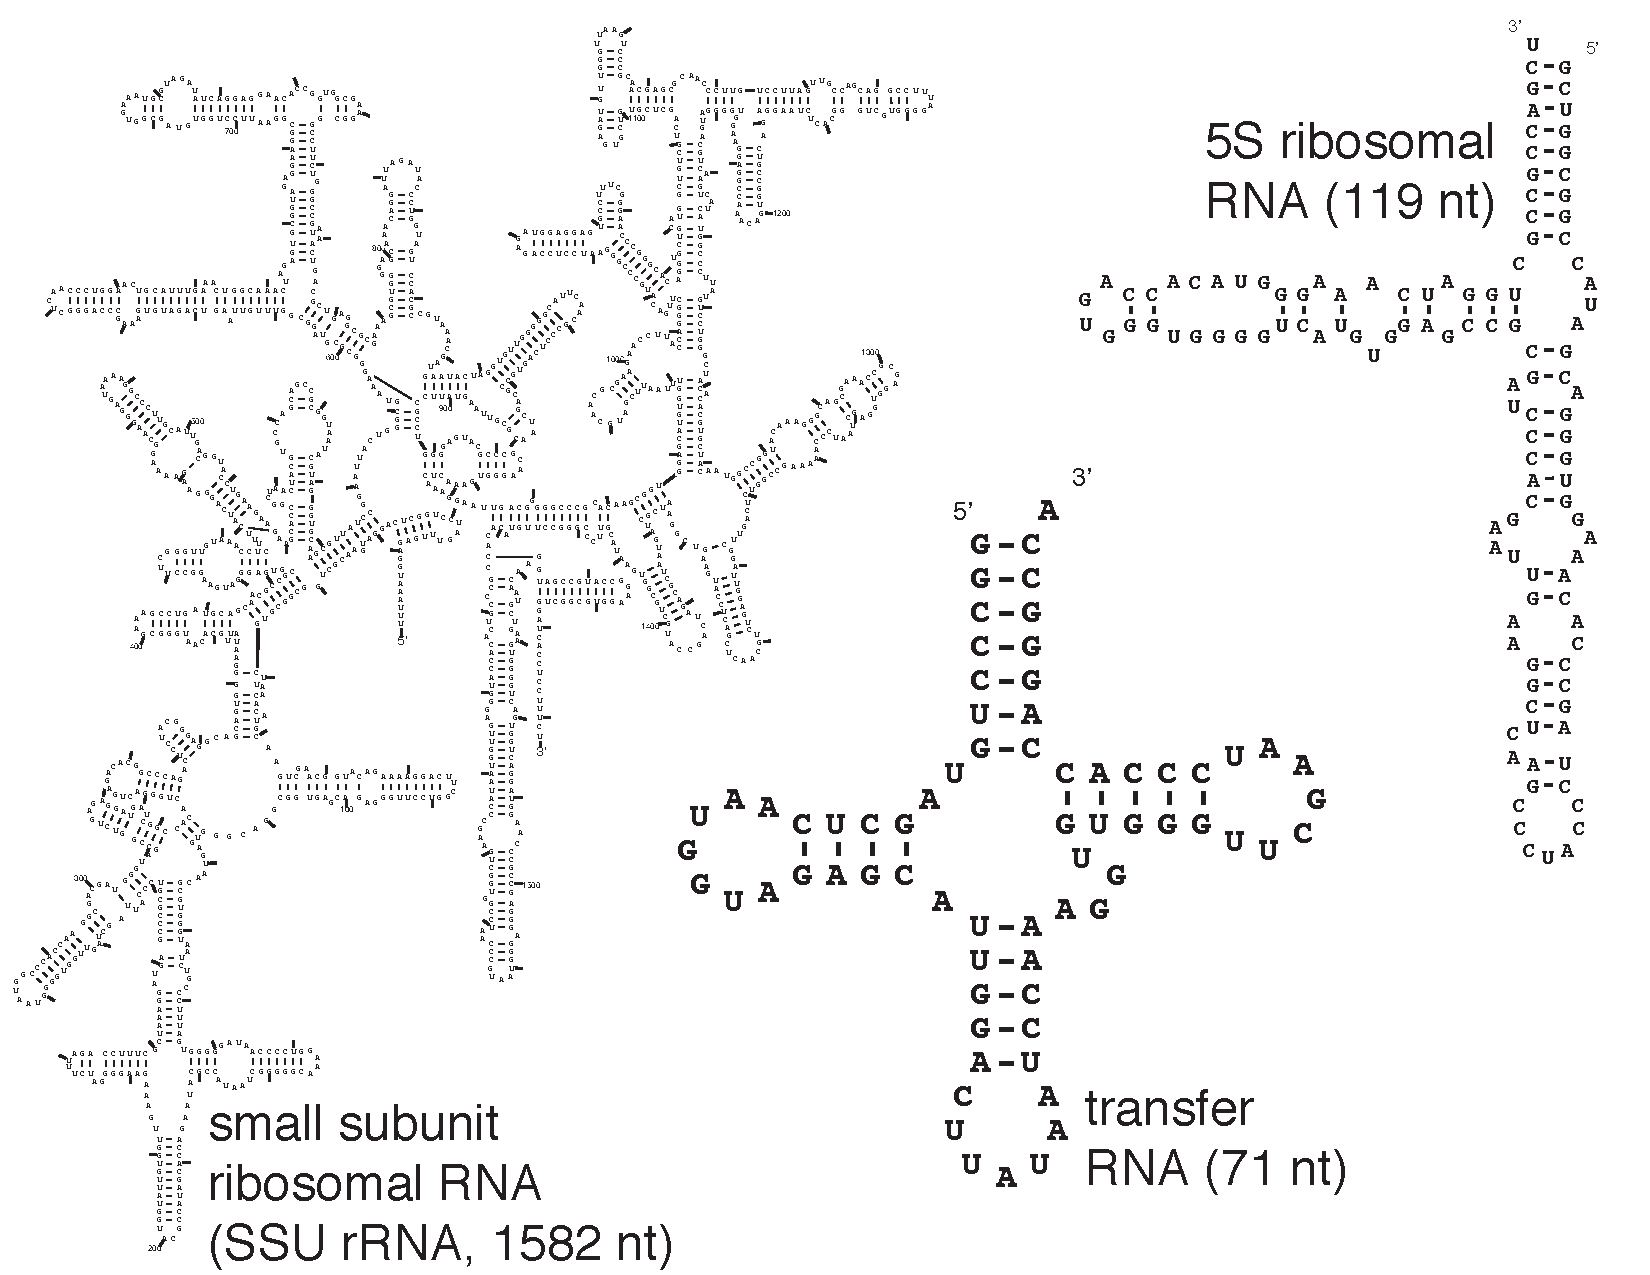
\includegraphics[width=10.5in]{figs/16s-5s-trna-allblack}}
\end{slide}
%%%%%%%%%%%%%%%%%%%%%%%%%%%%%%%%%%%%%%%%%%%%%%%%%%%%%%%%%%%%%%%%%%%%
\begin{slide}
\center{\includegraphics[width=10.5in]{figs/trna-covariation1}}
\end{slide}
%%%%%%%%%%%%%%%%%%%%%%%%%%%%%%%%%%%%%%%%%%%%%%%%%%%%%%%%%%%%%%%%%%%%
\begin{slide}
\center{\includegraphics[width=10.5in]{figs/trna-covariation2}}
\end{slide}
%%%%%%%%%%%%%%%%%%%%%%%%%%%%%%%%%%%%%%%%%%%%%%%%%%%%%%%%%%%%%%%%%%%%
%\begin{slide}
%\center{\includegraphics[width=10.5in]{figs/trna-covariation3a}}
%\end{slide}
%%%%%%%%%%%%%%%%%%%%%%%%%%%%%%%%%%%%%%%%%%%%%%%%%%%%%%%%%%%%%%%%%%%%
\begin{slide}
\center{\includegraphics[width=10.5in]{figs/trna-covariation3b}}
\end{slide}
%%%%%%%%%%%%%%%%%%%%%%%%%%%%%%%%%%%%%%%%%%%%%%%%%%%%%%%%%%%%%%%%%%%%
%\begin{slide}
%\center{\includegraphics[width=10.5in]{figs/trna-covariation4a}}
%\end{slide}
%%%%%%%%%%%%%%%%%%%%%%%%%%%%%%%%%%%%%%%%%%%%%%%%%%%%%%%%%%%%%%%%%%%%
\begin{slide}
\center{\includegraphics[width=10.5in]{figs/trna-covariation4b}}
\end{slide}
%%%%%%%%%%%%%%%%%%%%%%%%%%%%%%%%%%%%%%%%%%%%%%%%%%%%%%%%%%%%%%%%%%%%
\begin{slide}
\center{\includegraphics[width=10.5in]{figs/trna-covariation4c}}
\end{slide}
%%%%%%%%%%%%%%%%%%%%%%%%%%%%%%%%%%%%%%%%%%%%%%%%%%%%%%%%%%%%%%%%%%%%
%\begin{slide}
%\center{\includegraphics[width=10.5in]{figs/trna-covariation5a}}
%\end{slide}
%%%%%%%%%%%%%%%%%%%%%%%%%%%%%%%%%%%%%%%%%%%%%%%%%%%%%%%%%%%%%%%%%%%%
\begin{slide}
\center{\includegraphics[width=10.5in]{figs/trna-covariation5b}}
\end{slide}
%%%%%%%%%%%%%%%%%%%%%%%%%%%%%%%%%%%%%%%%%%%%%%%%%%%%%%%%%%%%%%%%%%%%
\begin{slide}
\center{\includegraphics[width=10.5in]{figs/trna-covariation5c}}
\end{slide}
%%%%%%%%%%%%%%%%%%%%%%%%%%%%%%%%%%%%%%%%%%%%%%%%%%%%%%%%%%%%%%%%%%%%
\begin{slide}
\center{\includegraphics[width=10.5in]{figs/trna-covariation3b}}
\end{slide}
%%%%%%%%%%%%%%%%%%%%%%%%%%%%%%%%%%%%%%%%%%%%%%%%%%%%%%%%%%%%%%%%%%%%
\begin{slide}
\center{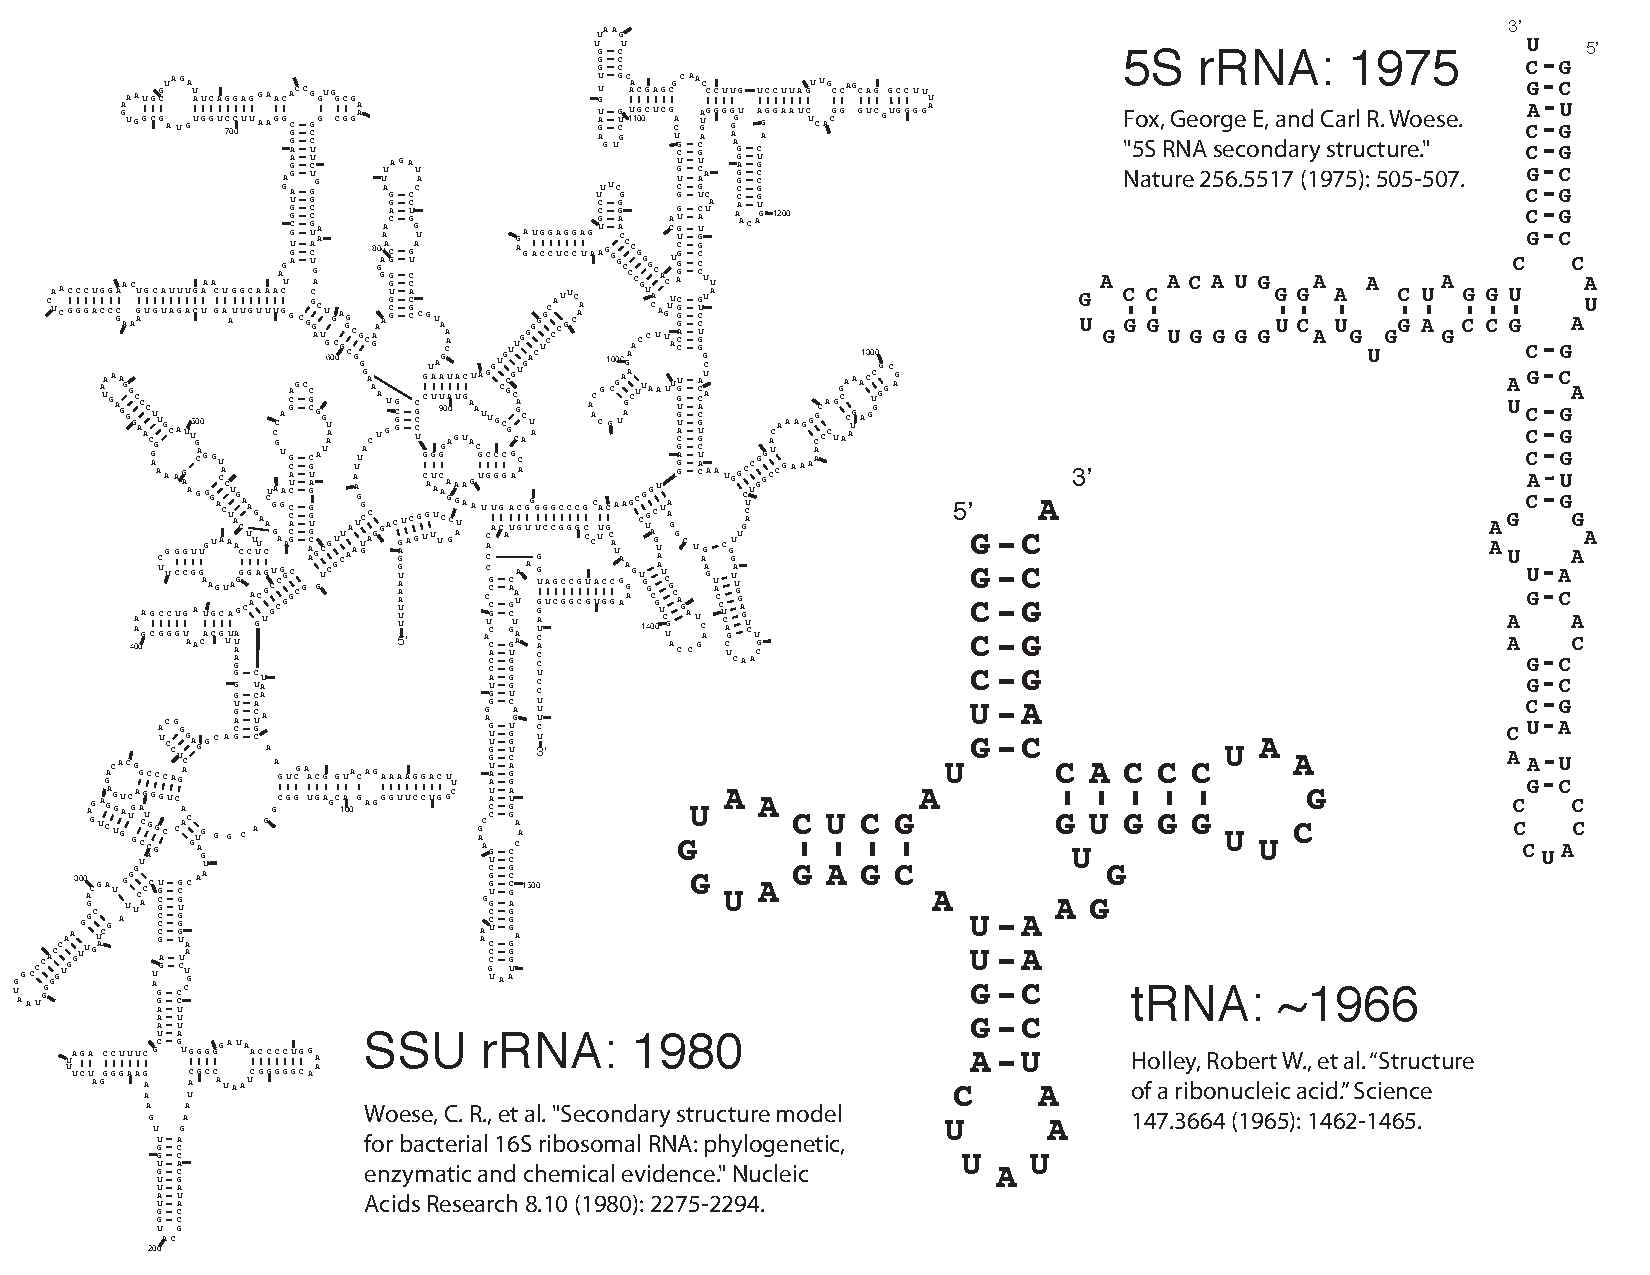
\includegraphics[width=10.5in]{figs/16s-5s-trna-allblack-dates-refs}}
\end{slide}
%%%%%%%%%%%%%%%%%%%%%%%%%%%%%%%%%%%%%%%%%%%%%%%%%%%%%%%%%%%%%%%%%%%%
%\begin{slide}
%\center{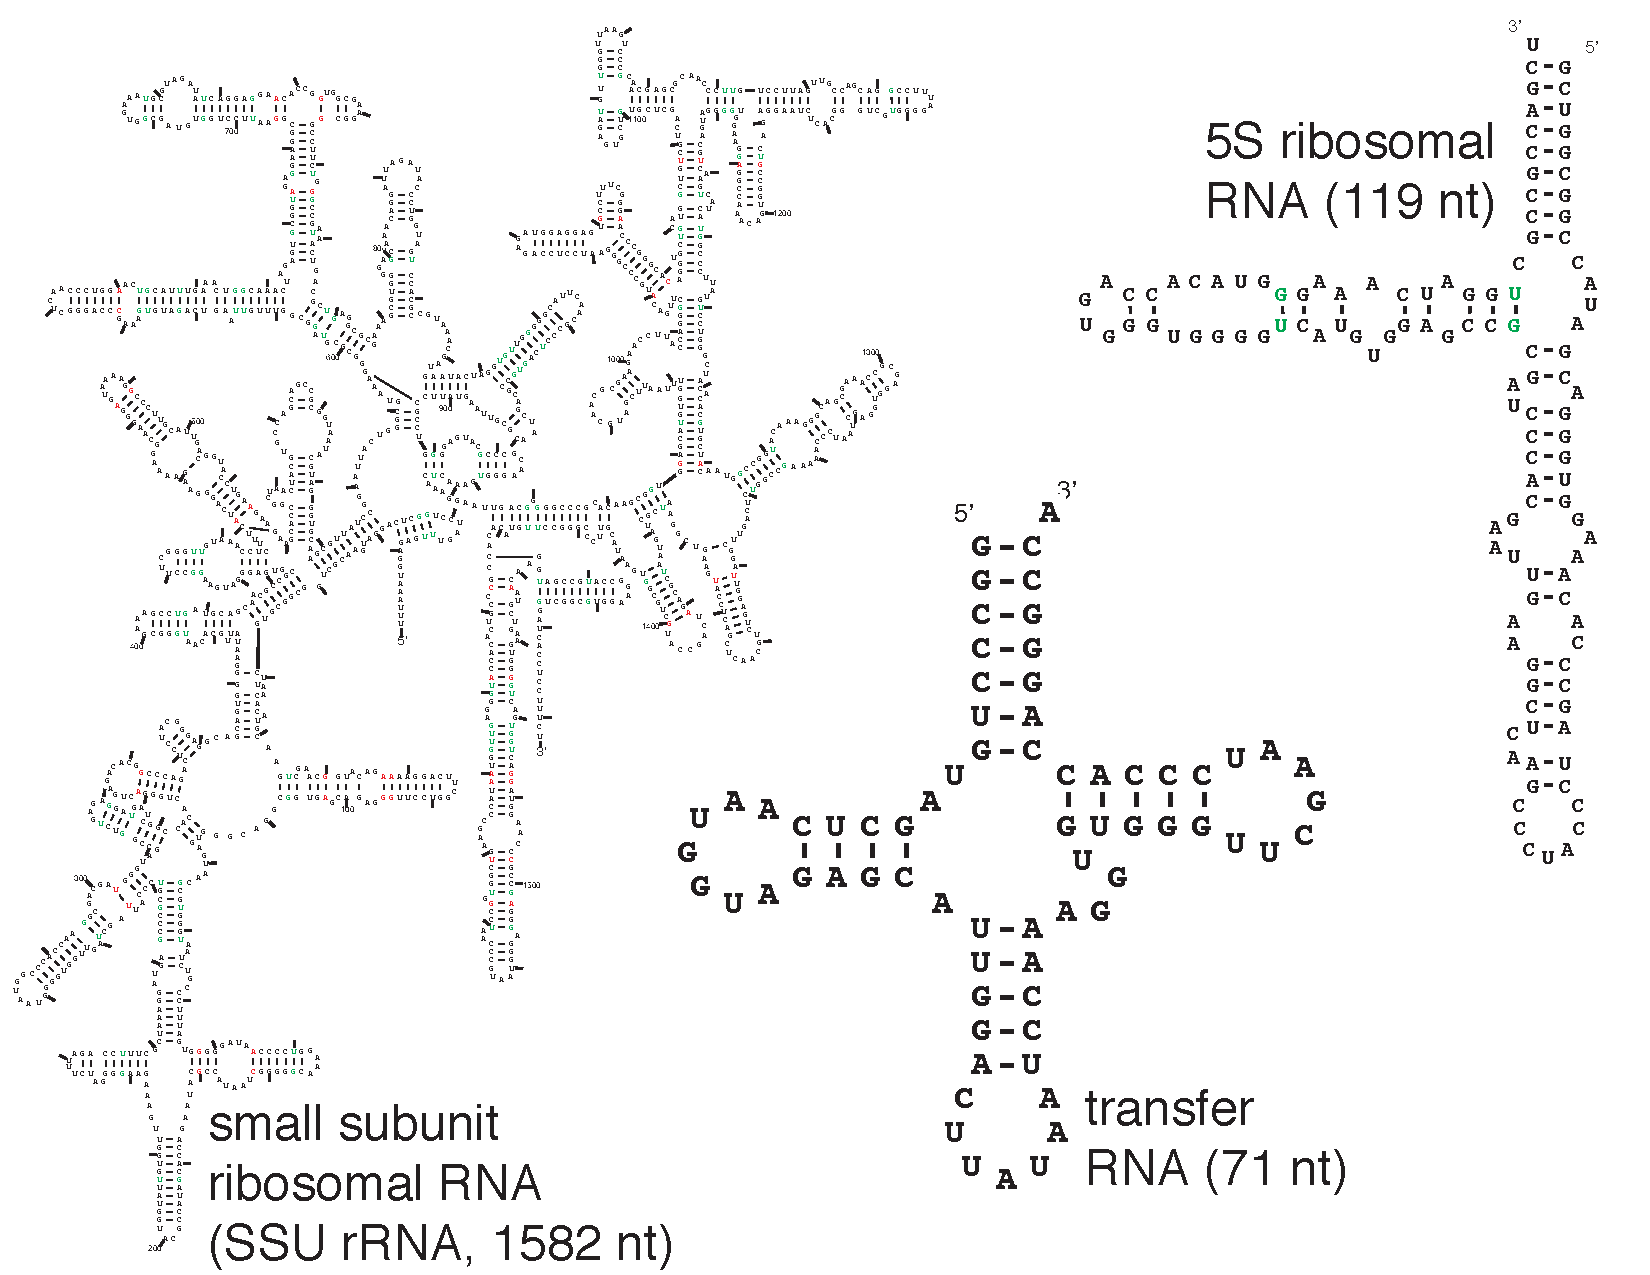
\includegraphics[width=10.5in]{figs/16s-5s-trna-bpcolored}}
%\end{slide}
%%%%%%%%%%%%%%%%%%%%%%%%%%%%%%%%%%%%%%%%%%%%%%%%%%%%%%%%%%%%%%%%%%%%
\begin{slide}

\center{\textbf{Comparative sequence analysis informs biologists}}

\small
\begin{itemize}
\item What we can learn about the gene family being studied:
\begin{itemize}
  \item structure
  \item conservation suggests functional importance 
\end{itemize}
\end{itemize}

\vfill
\end{slide}
%%%%%%%%%%%%%%%%%%%%%%%%%%%%%%%%%%%%%%%%%%%%%%%%%%%%%%%%%%%%%%%%%%%%
\begin{slide}
\center{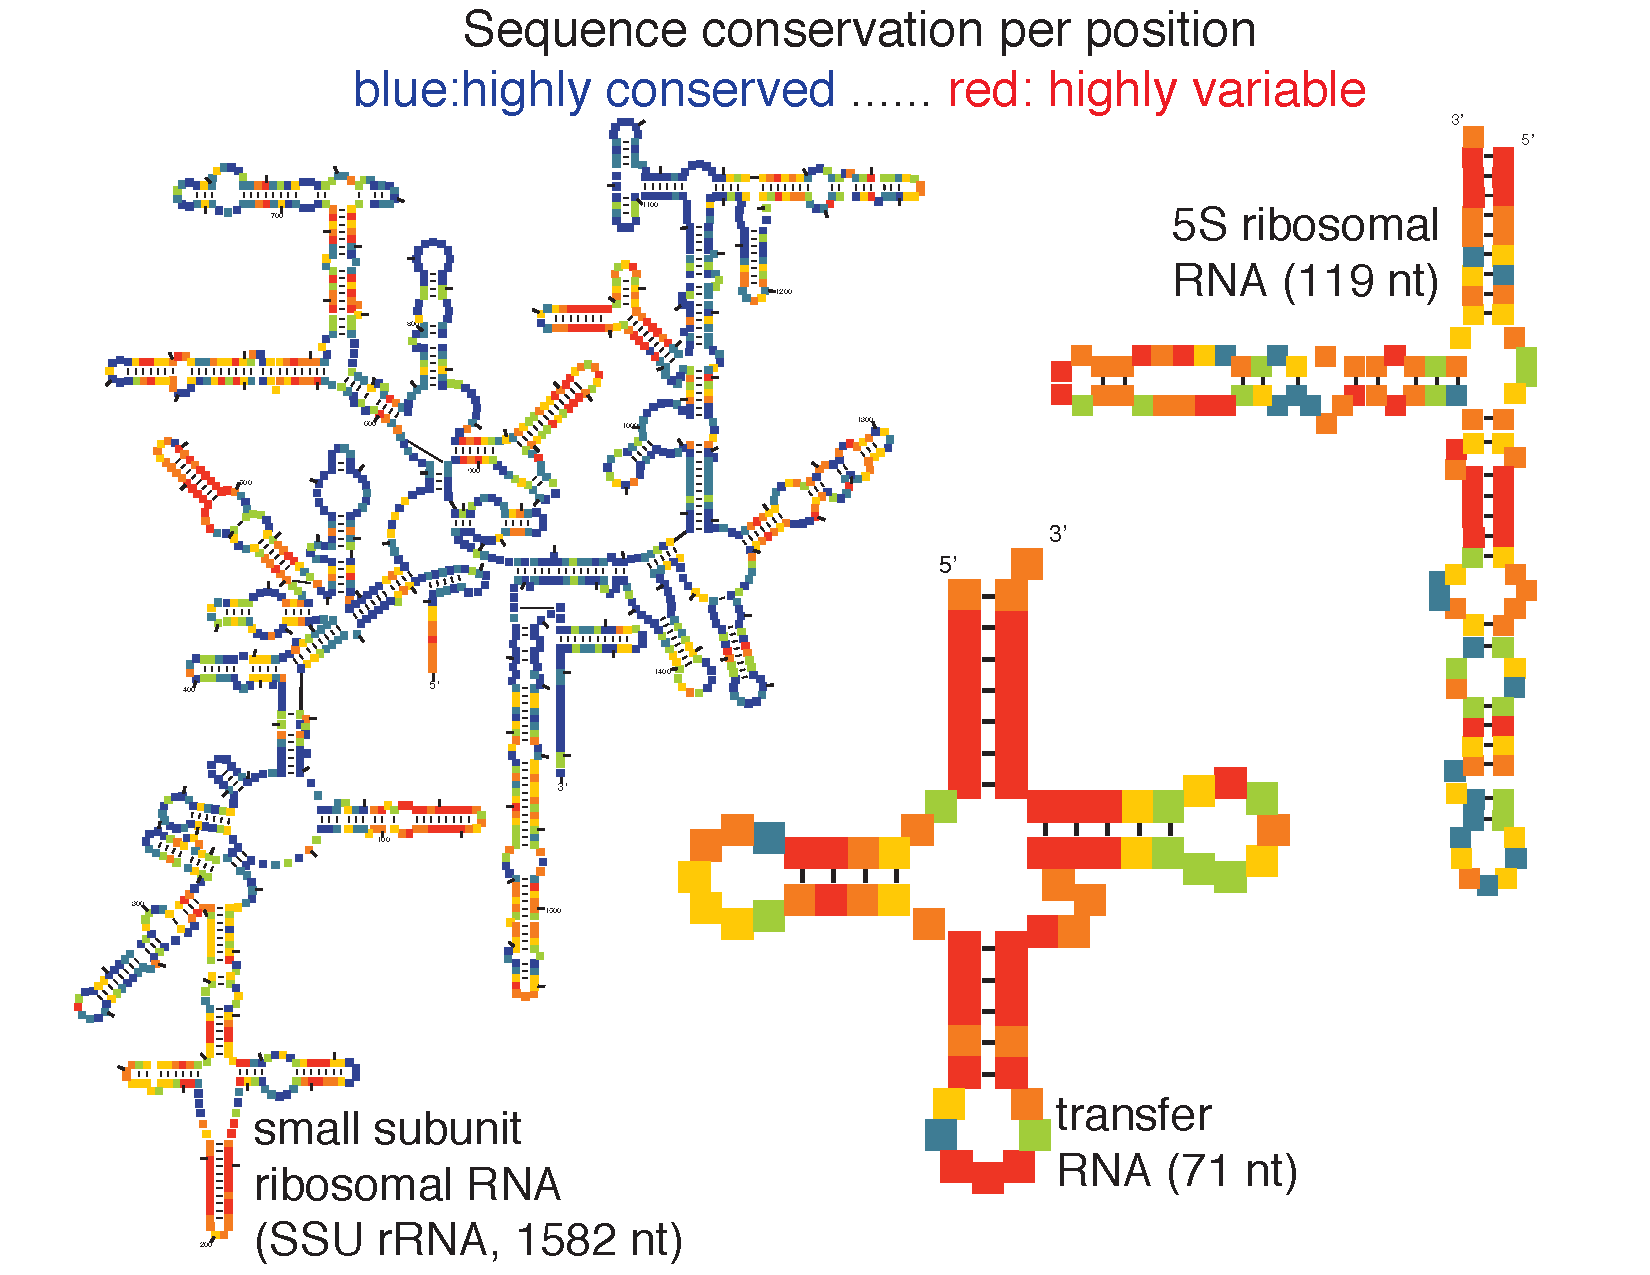
\includegraphics[width=10.5in]{figs/16s-5s-trna-info}}
\end{slide}
%%%%%%%%%%%%%%%%%%%%%%%%%%%%%%%%%%%%%%%%%%%%%%%%%%%%%%%%%%%%%%%%%%%%
\begin{slide}

\center{\textbf{Comparative sequence analysis informs biologists}}

\small
\begin{itemize}
\item What we can learn about the gene family being studied:
\begin{itemize}
  \item structure
  \item conservation suggests functional importance
\end{itemize}

\item What we can learn about organism/environment sequences derive
  from:
\begin{itemize}
  \item which biological processes are being carried out
  \item phylogenetic placement
\end{itemize}
\end{itemize}

\vfill
\end{slide}
%%%%%%%%%%%%%%%%%%%%%%%%%%%%%%%%%%%%%%%%%%%%%%%%%%%%%%%%%%%%%%%%%%%%
\begin{slide}

\center{\textbf{Comparative sequence analysis informs biologists}}

\small
\begin{itemize}
\item What we can learn about the gene family being studied:
\begin{itemize}
  \item structure
  \item conservation suggests functional importance
\end{itemize}

\item What we can learn about organism/environment sequences derive
  from:
\begin{itemize}
  \item which biological processes are being carried out
  \item phylogenetic placement
\end{itemize}
\end{itemize}

\normalsize
\begin{center}
Comparative analysis requires multiple gene family examples
(homologs).

\textcolor{red}{Computational \emph{homology search} methods use \\ one or more known
family members to find additional homologs.}
\end{center}

\vfill
\end{slide}
%%%%%%%%%%%%%%%%%%%%%%%%%%%%%%%%%%%%%%%%%%%%%%%%%%%%%%%%%%%%%%%%%%%%
%\begin{slide}
%
%\center{\textbf{Key advances in homology search}}
%
%\small
%\begin{itemize}
%\item 1970-1974: Needleman, Wunsch and Sellers develop an $O(N^2)$algorithm for aligning two
%  sequences 
%\item 1981: Smith and Waterman devise a local alignment algorithm.
%\item 1987: Gribskov et al. introduce profile models with position
%  specific scoring systems.
%\item 1990: BLAST is published: a tool for fast sequence homology
%  searches, a heuristic of Smith/Waterman
%\item 1994: Krogh and Haussler introduce probabilistic profiles called
%  profile hidden Markov models (profile HMMs)
%\end{itemize}
%
%\vfill
%\end{slide}
%%%%%%%%%%%%%%%%%%%%%%%%%%%%%%%%%%%%%%%%%%%%%%%%%%%%%%%%%%%%%%%%%%%%
\begin{slide}
\begin{center}
%\textbf{Comparative analysis of sequence families}: \\
\textbf{Sequence conservation provides \\ information for homology searches}
%\emph{Functionally important sequence features are evolutionarily conserved.}
\medskip

%A simple, made-up RNA family:

%Evolution conserves functionally \\ important sequence features.

%Evolution conserves sequence \\ based on its functional importance.

Conservation levels vary across alignment columns.

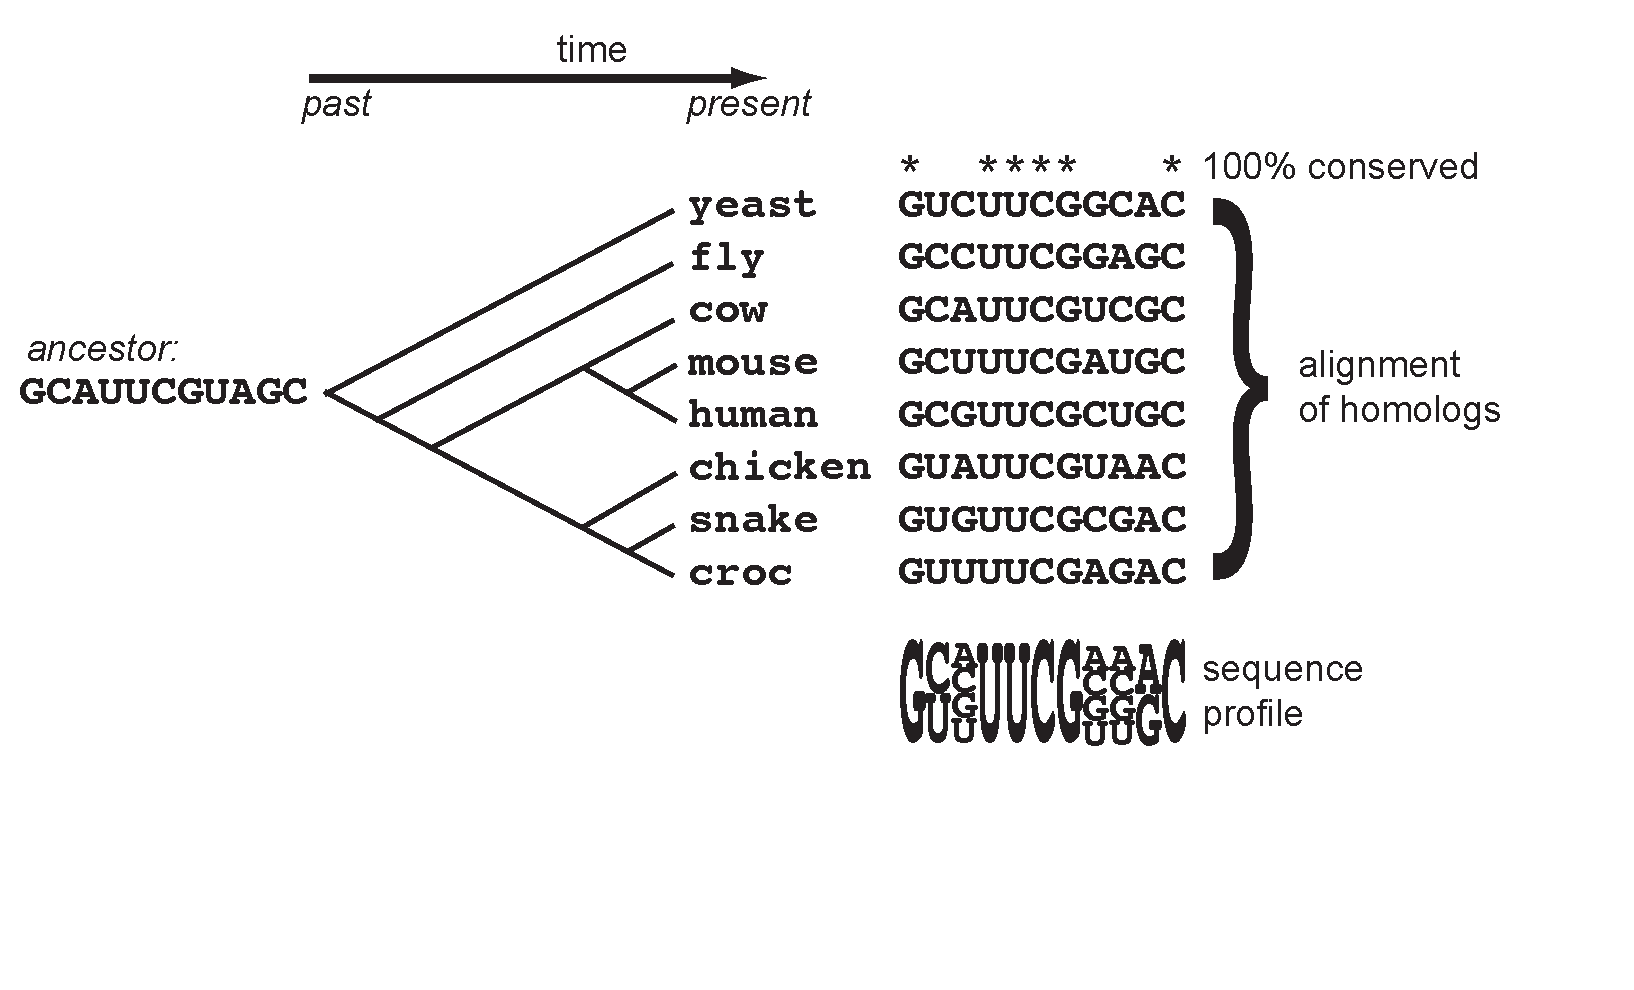
\includegraphics[width=8.625in]{figs/seqstructprofiles-seq1}
\end{center}

\vfill
\end{slide}
%%%%%%%%%%%%%%%%%%%%%%%%%%%%%%%%%%%%%%%%%%%%%%%%%%%%%%%%%%%%%%%%%%%%%%
\begin{slide}
\begin{center}
\textbf{Structure conservation provides additional information}
\medskip

Base-paired positions covary \\ to maintain Watson-Crick complementarity.

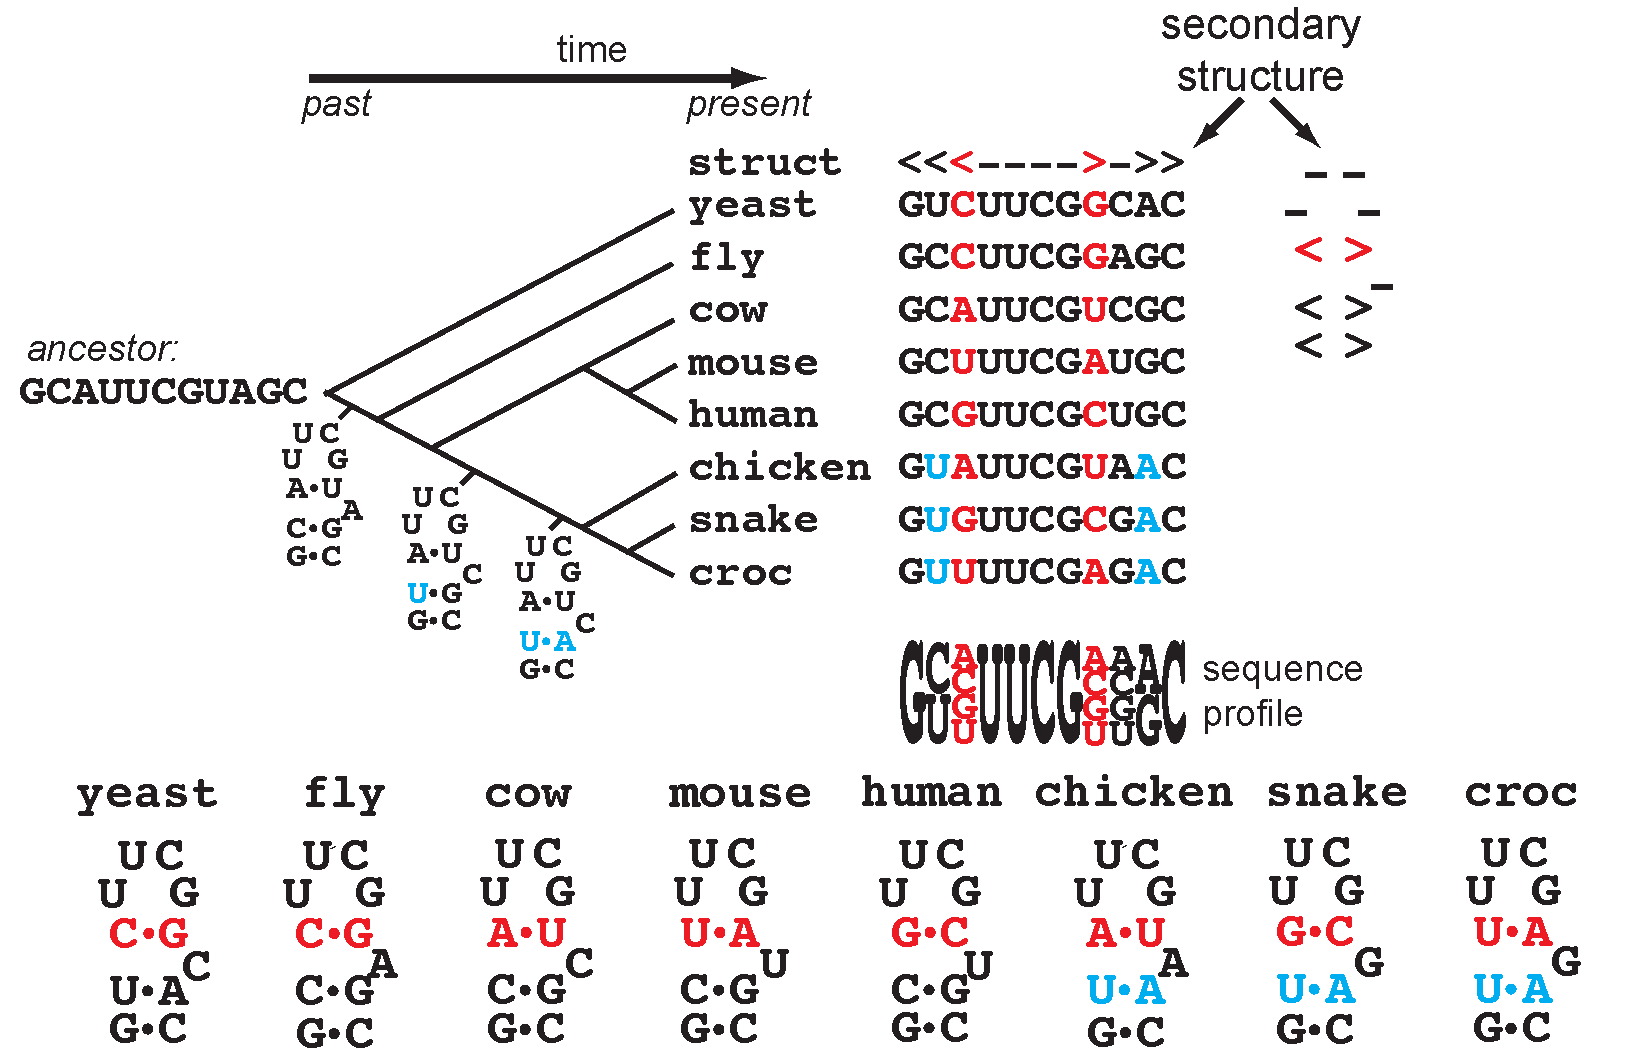
\includegraphics[width=8.625in]{figs/seqstructprofiles-struct2}
\end{center}

\vfill
\end{slide}
%%%%%%%%%%%%%%%%%%%%%%%%%%%%%%%%%%%%%%%%%%%%%%%%%%%%%%%%%%%%%%%%%%%%%%%%%%
\begin{slide}
\begin{center}
\textbf{Levels of sequence and structure conservation in RNA families}
\end{center}
\medskip

\begin{center}
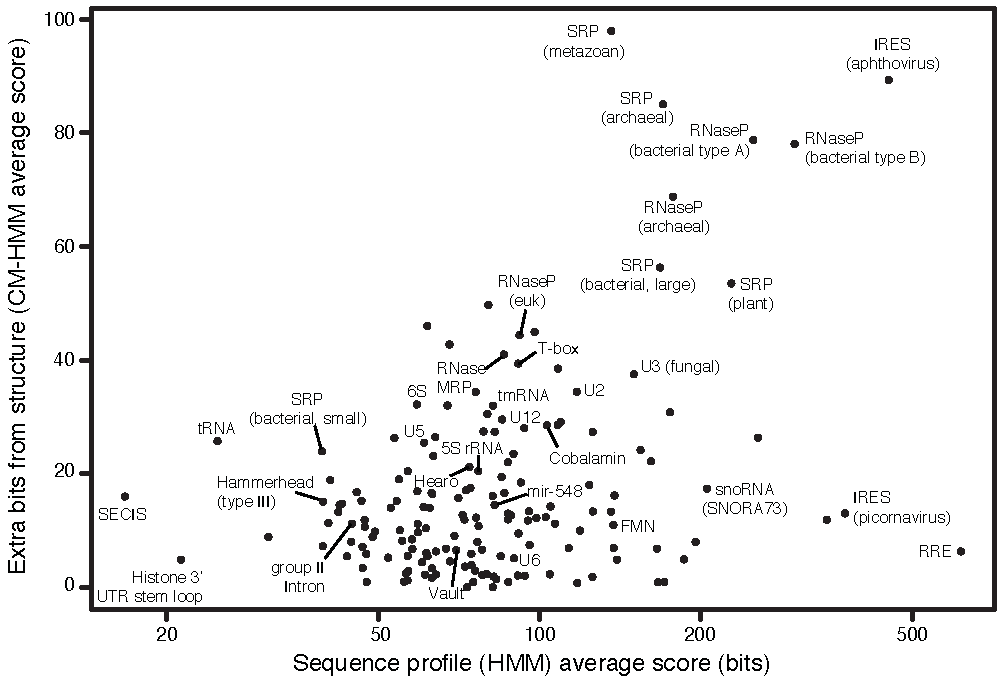
\includegraphics[height=6.5in]{figs/avgscores-rfam11}
\end{center}

\vfill

\end{slide}
%%%%%%%%%%%%%%%%%%%%%%%%%%%%%%%%%%%%%%%%%%%%%%%%%%%%%%%%%%%%%%%%%%%
\begin{slide}
\begin{center}
%\textbf{profile HMMs and covariance models}
\textbf{Eddy lab software for profile probabilistic models} (since 1994)
\end{center}
\medskip

\begin{center}
\small
\begin{tabular}{r|cc} 
%             &         & sequence \\
%             & sequence& and structure \\
%             & profiles& profiles \\ \hline
             & sequence & sequence and \\
             & profiles & structure profiles \\ \hline
  \\
  models     & profile HMMs     & {\color{red} covariance models (CMs)} \\ 
  \\
  software   & {\sc HMMER}      & {\sc Infernal} \\ 
  \\
  main use   & proteins         & RNAs \\ 
  \\
  database   & {\sc Pfam}       & {\sc Rfam} \\
             & (14831 families) & (2208 families) \\
  \\
%  primary sequence & yes & yes \\
%  \\
%  secondary structure & no & yes \\
%  \\
%  algorithms & Viterbi, Forward & CYK, Inside \\
%%             & Forward & Inside \\
%             &         & \\
%  complexity & $O(LN)$ & $O(LN^{2} log N)$ \\
%  \\
  performance& faster but    & slower but    \\
  for RNAs   & less accurate & more accurate \\
\end{tabular}

%\hspace{1.2in}
\includegraphics[height=2in]{figs/hmmer_logo}\hspace{1.05in}
\includegraphics[height=2.6in]{figs/infernal_logo}
\hspace{1.2in}
\includegraphics[height=2.8in]{figs/hmmer-infernal-refs}

\end{center}

\vfill

\end{slide}
%%%%%%%%%%%%%%%%%%%%%%%%%%%%%%%%%%%%%%%%%%%%%%%%%%%%%%%%%%%%%%%%%%%%
\begin{slide}
\begin{center}
\textbf{Profile HMMs: sequence family models built from alignments}
\end{center}
\center{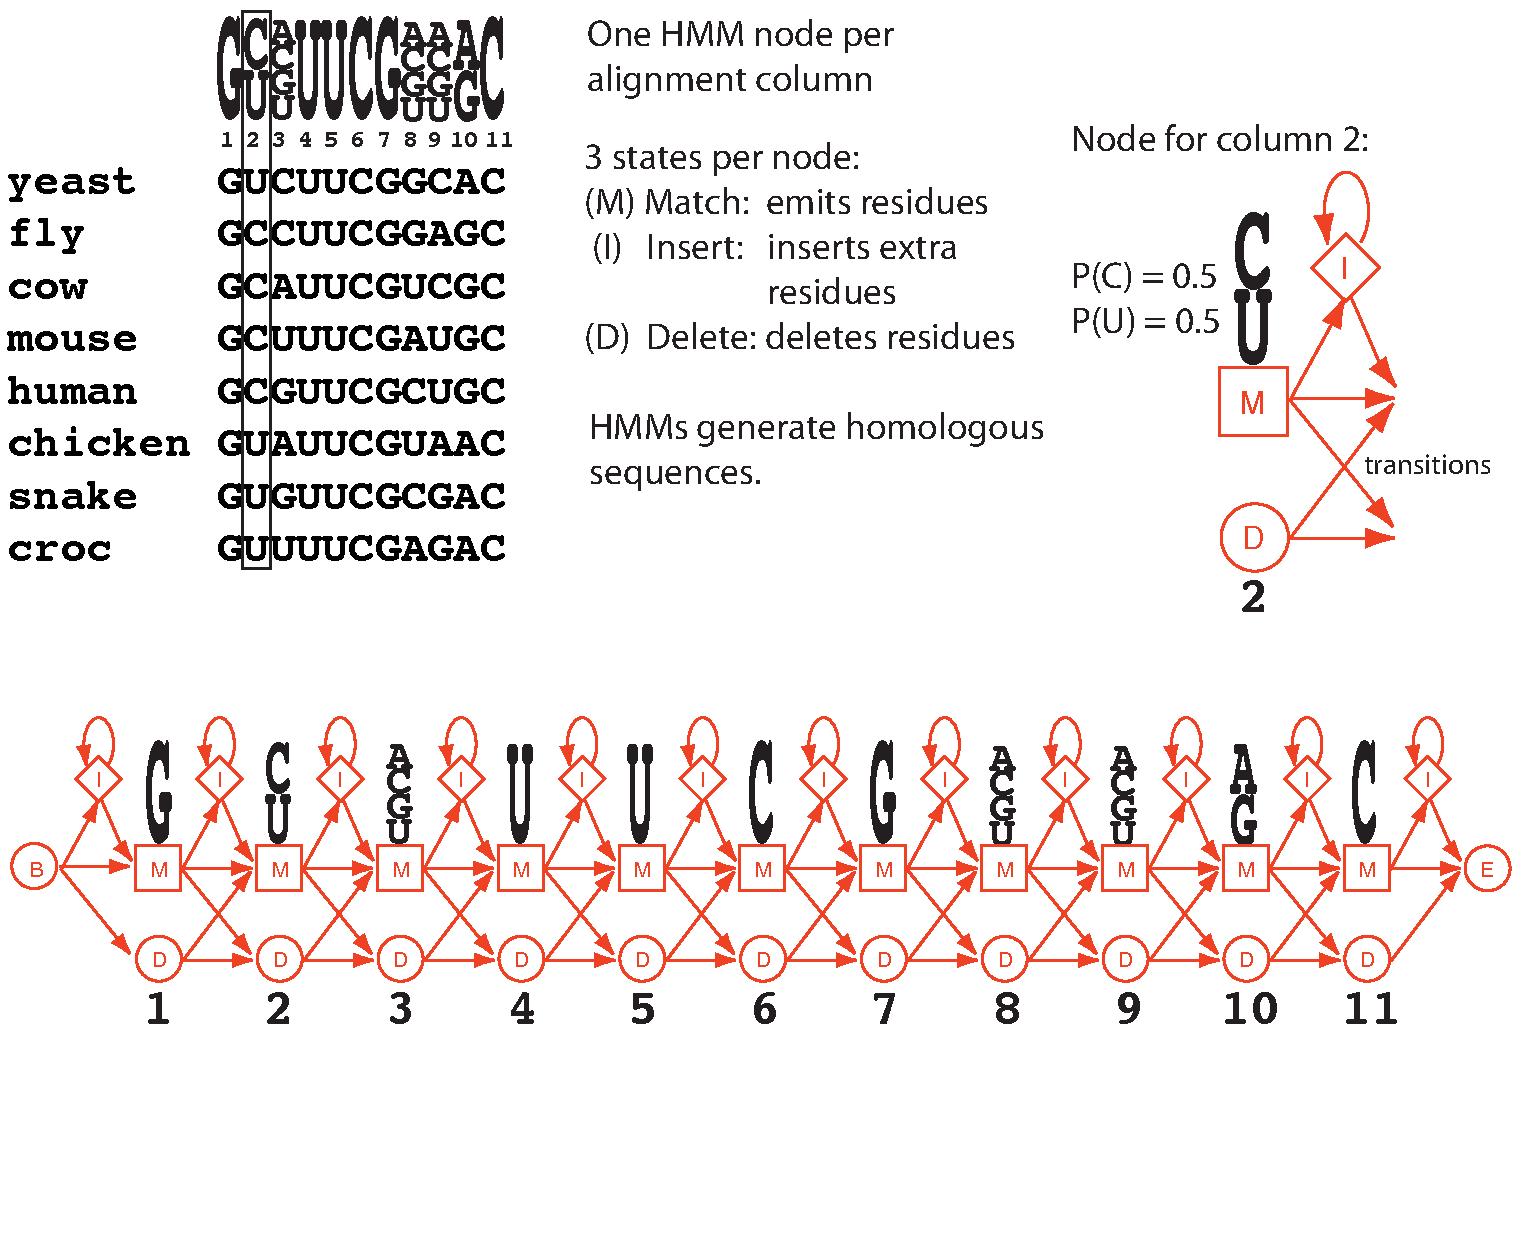
\includegraphics[height=6.625in]{figs/hmm}}
\end{slide}
%%%%%%%%%%%%%%%%%%%%%%%%%%%%%%%%%%%%%%%%%%%%%%%%%%%%%%%%%%%%%%%
\begin{slide}
\begin{center}
\textbf{Profile HMMs: sequence family models built from alignments}
\end{center}
\center{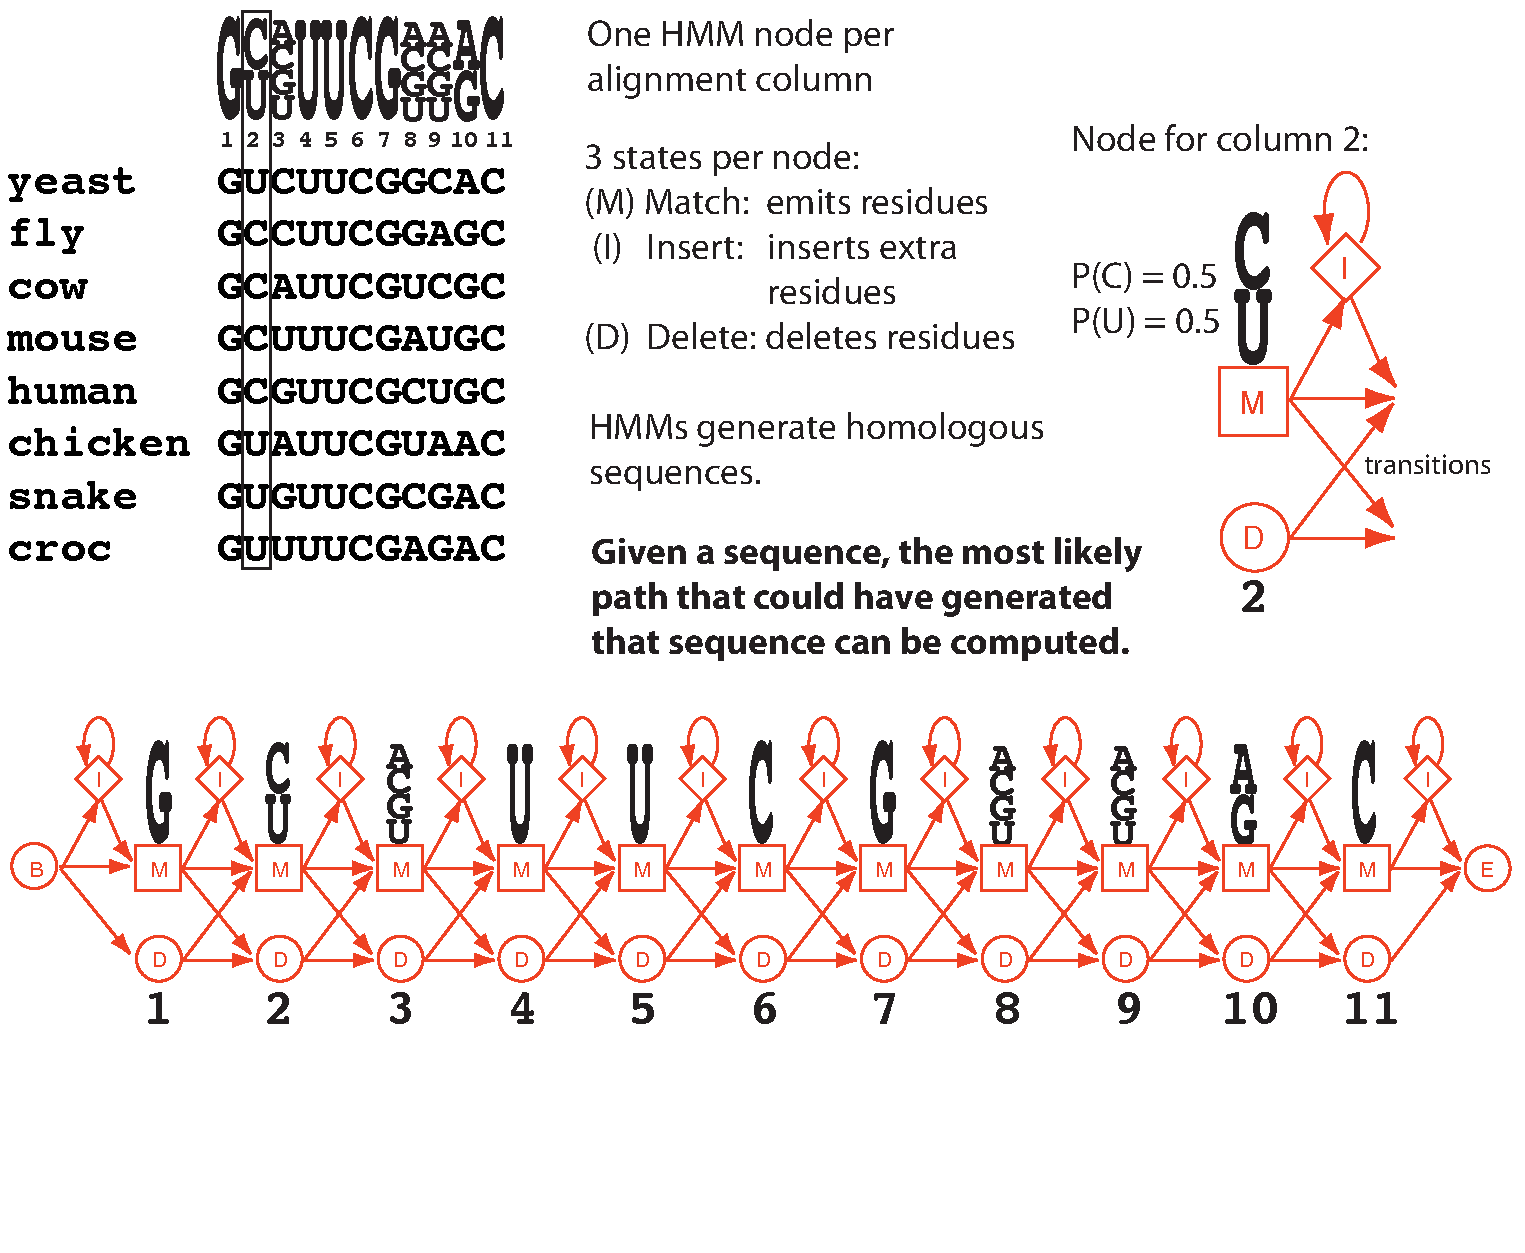
\includegraphics[height=6.625in]{figs/hmm-given}}
\end{slide}
%%%%%%%%%%%%%%%%%%%%%%%%%%%%%%%%%%%%%%%%%%%%%%%%%%%%%%%%%%%%%%%
\begin{slide}
\begin{center}
\textbf{Profile HMMs: sequence family models built from alignments}
\end{center}
\center{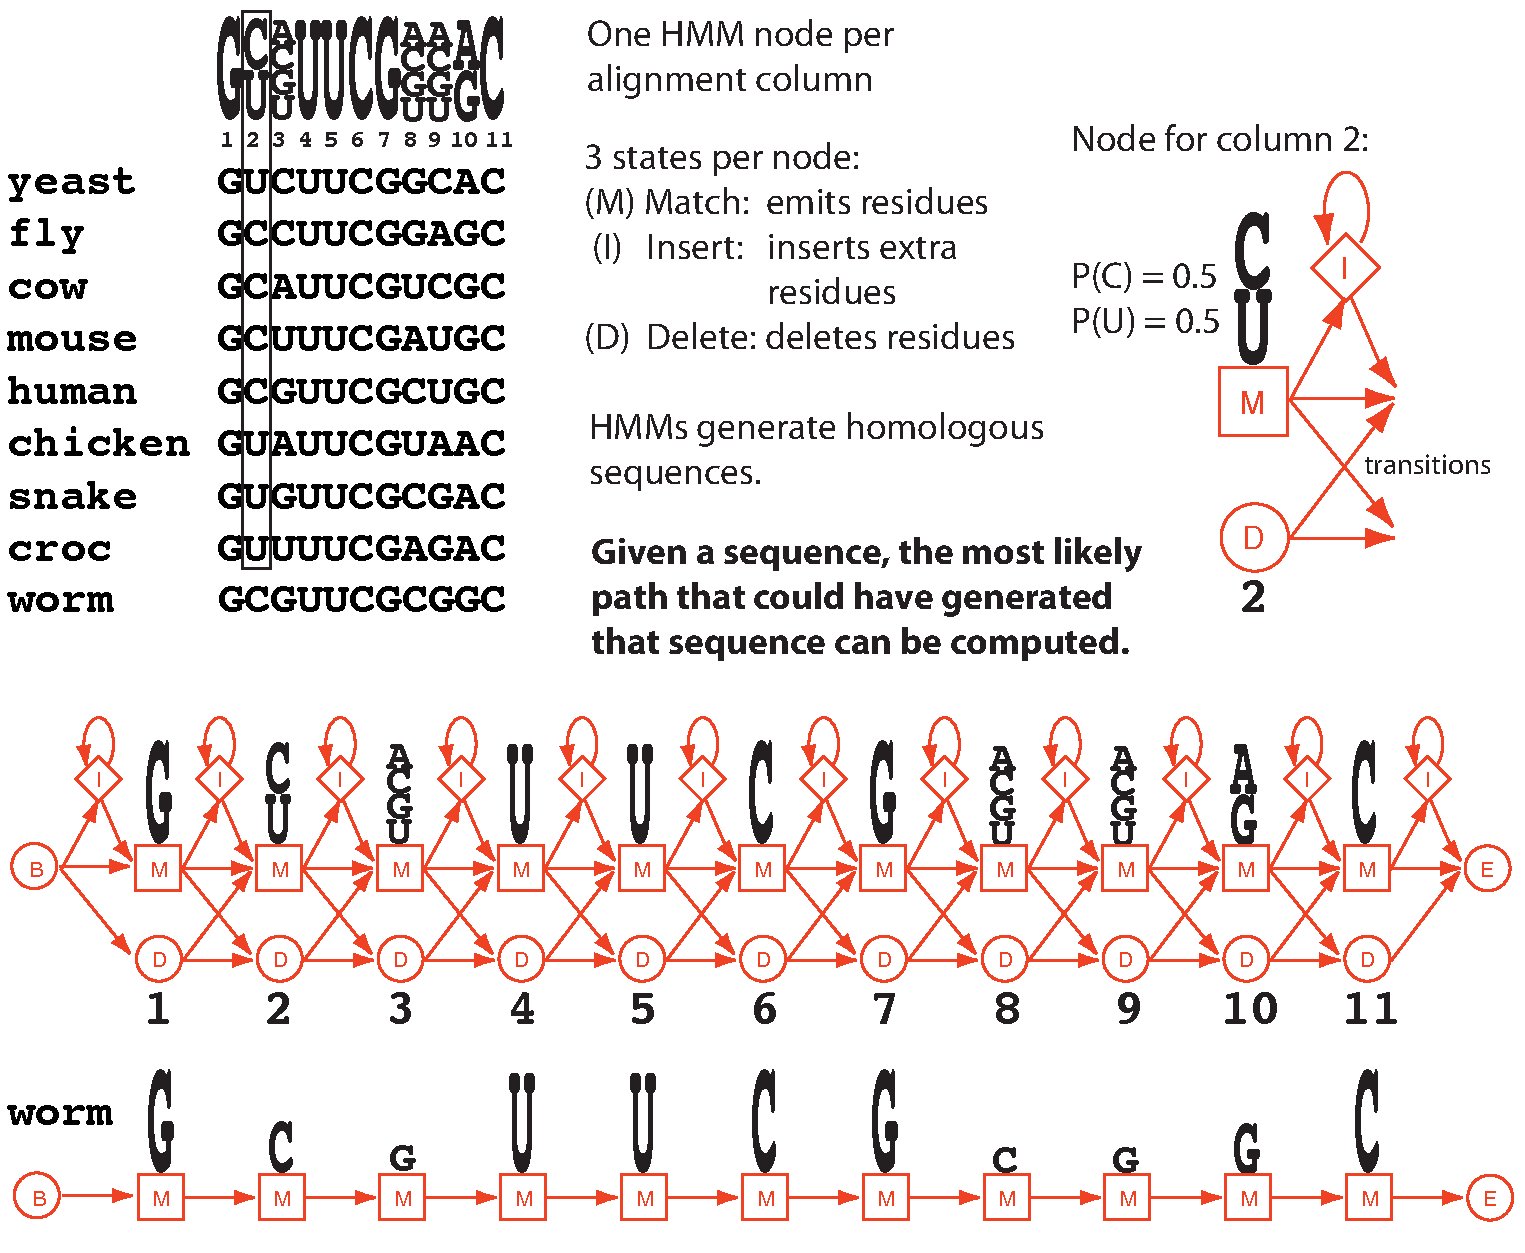
\includegraphics[height=6.625in]{figs/hmm-worm}}
\end{slide}
%%%%%%%%%%%%%%%%%%%%%%%%%%%%%%%%%%%%%%%%%%%%%%%%%%%%%%%%%%%
\begin{slide}
\begin{center}
\textbf{Profile HMMs: sequence family models built from alignments}
\end{center}
\center{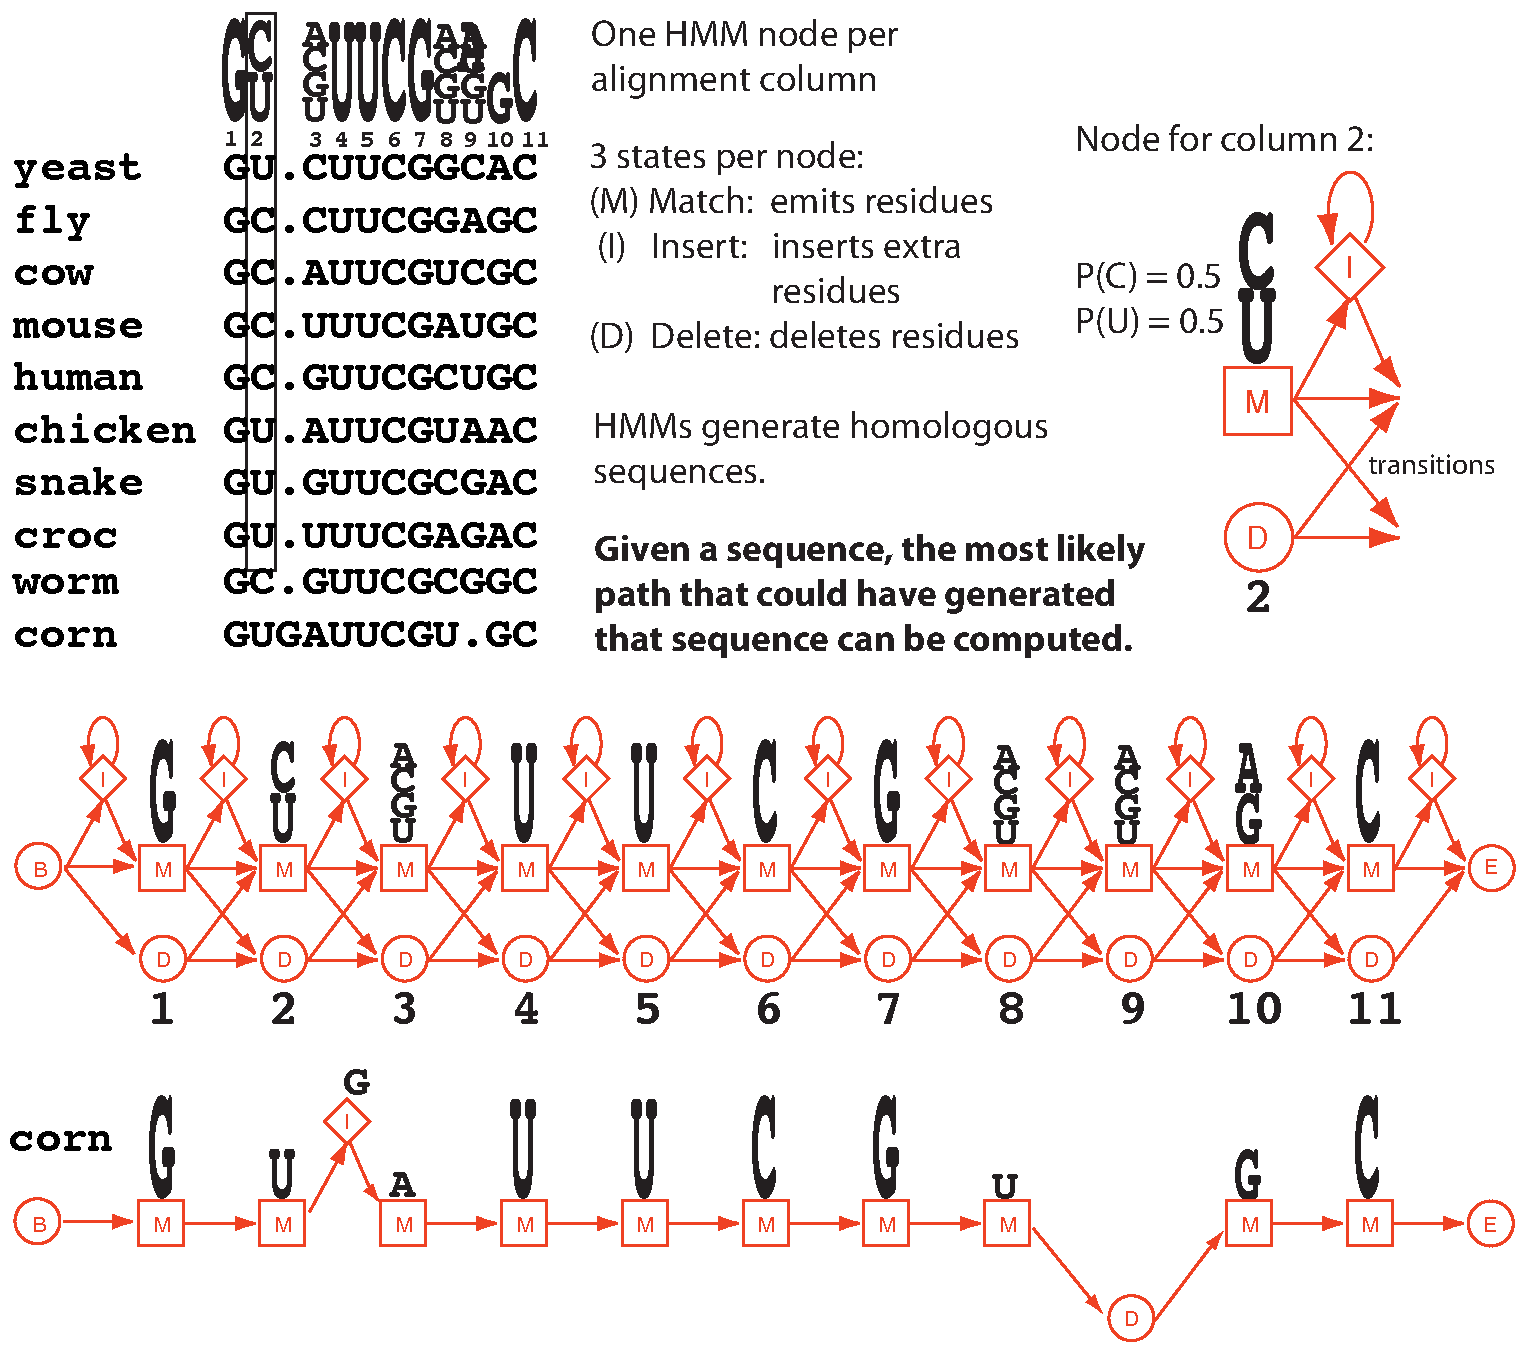
\includegraphics[height=6.625in]{figs/hmm-corn}}
\end{slide}
%%%%%%%%%%%%%%%%%%%%%%%%%%%%%%%%%%%%%%%%%%%%%%%%%%%%%%%%%%%%%%%
\begin{slide}
\begin{center}
\textbf{Covariance models (CMs) are built \\ from structure-annotated alignments}
\end{center}

\center{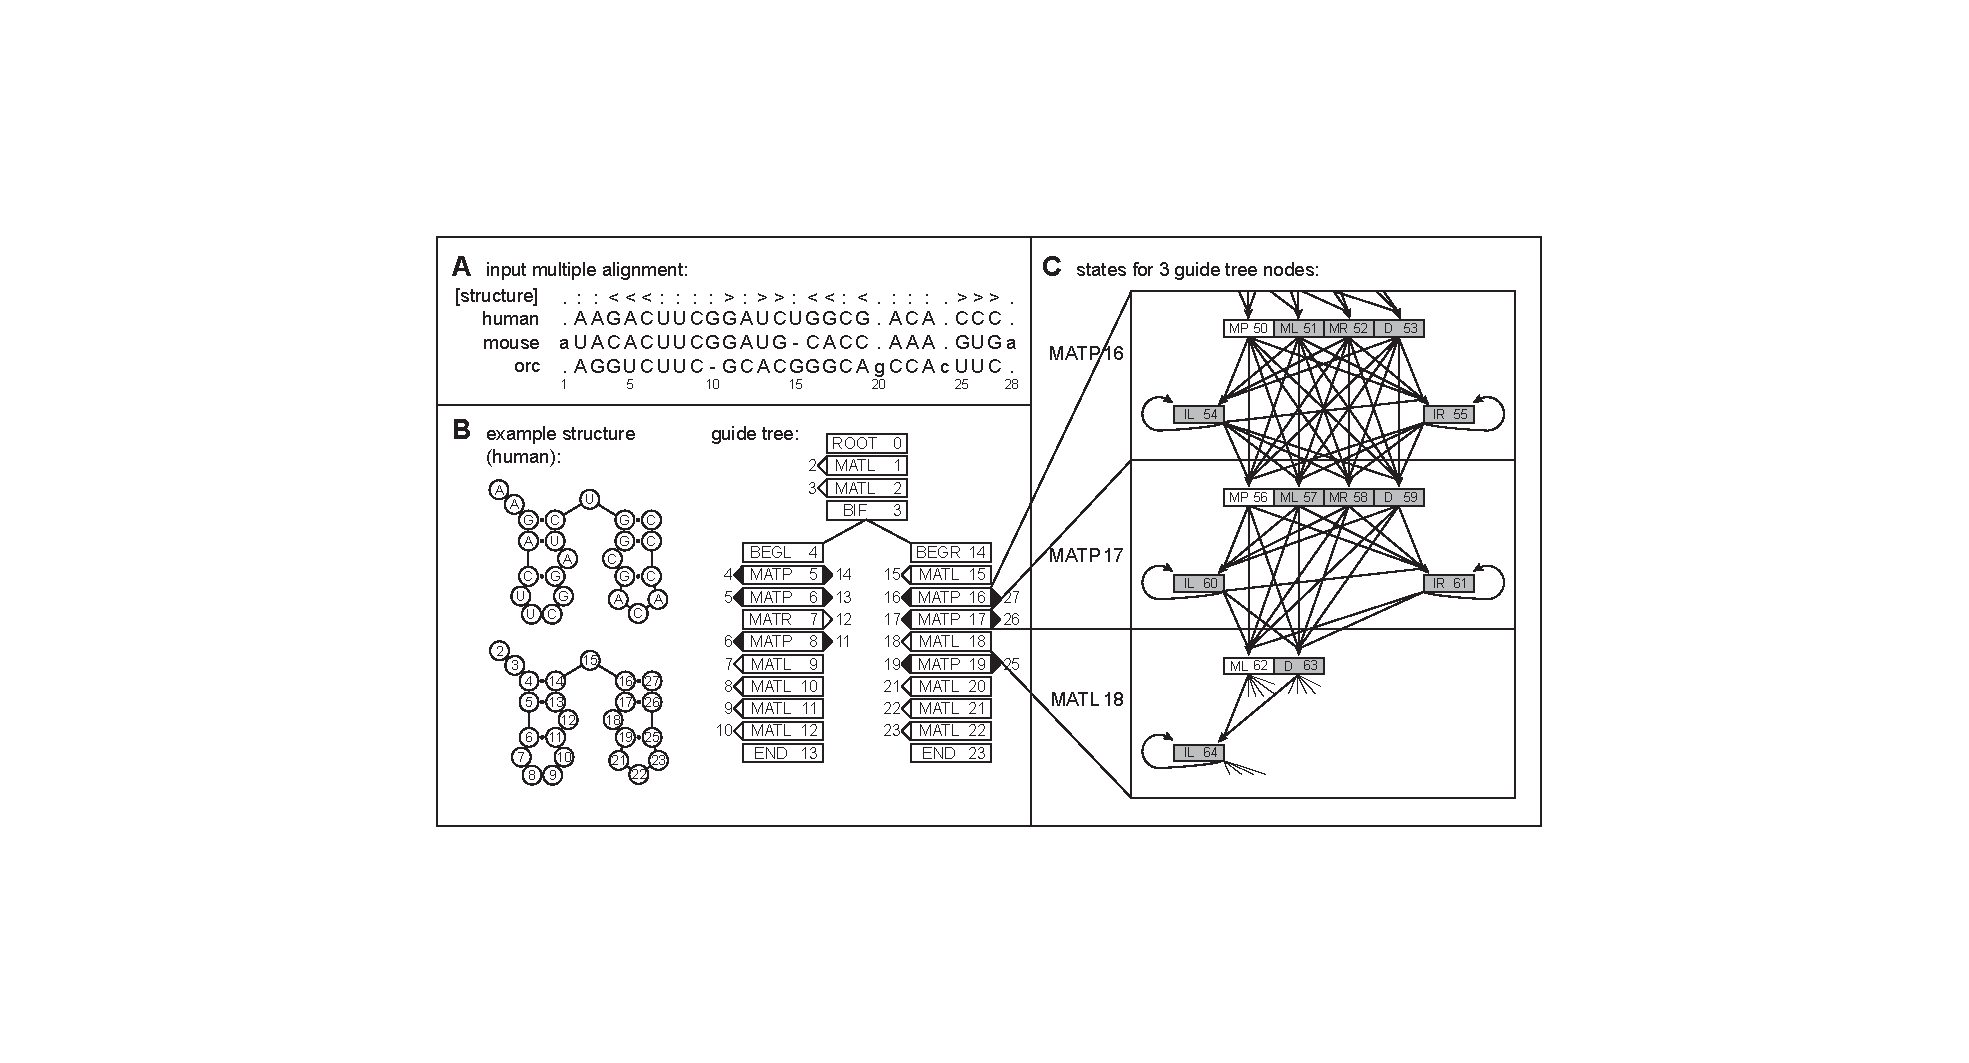
\includegraphics[width=7in]{figs/cmintro_bandcyk}}

\center{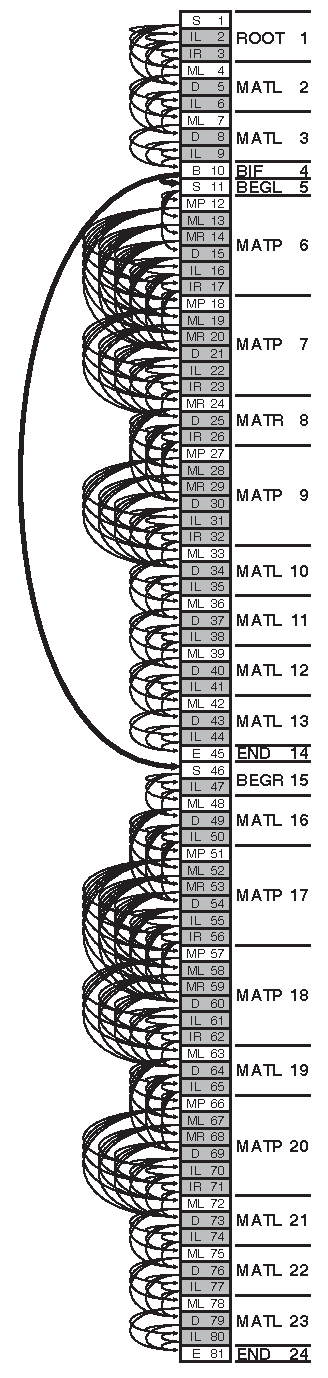
\includegraphics[width=2in,angle=270]{figs/cm-graph-small}}

\vfill
\end{slide}
%%%%%%%%%%%%%%%%%%%%%%%%%%%%%%%%%%%%%%%%%%%%%%%%%%%%%%%%%%%%%%%%%%
\begin{slide}
\begin{center}
\textbf{Is the added complexity worth it? \\
  RMARK: a challenging \underline{internal} RNA homology search \\
  benchmark for use during Infernal development}
\end{center}
\medskip
\begin{minipage}{7in}
\small
\begin{itemize}
\item
  RMARK construction - for each of the 1446 Rfam 10 seed alignments:
  \begin{itemize}
%  \item
%    remove sequences $<$ 70\% average family length
  \item 
    cluster sequences by sequence identity \\ given the alignment
  \item 
    look for a \textcolor{blue}{training} cluster and
    \textcolor{red}{testing} cluster such that: 
    \begin{itemize}
    \item
      no \textcolor{blue}{training}/\textcolor{red}{test} sequence pair is $>$ 60\% identical
    \item
      at least five sequences are in the \textcolor{blue}{training} set
    \end{itemize}
  \item
    filter \textcolor{red}{test} set so no two test seqs $>$ 70\% identical 
  \item
    %51 families qualify, with 450 \textcolor{red}{test} sequences
    106 families qualify, with 780 test sequences
  \item
    %\textcolor{red}{test} seqs are embedded in a 1 Mb pseudo-genome (25\% A,C,G,U)
    test seqs are embedded in a 10 Mb pseudo-genome of ``realistic'' base composition
%  \item
%    %    \textsc{BLAST}: family-pairwise search, each \textcolor{blue}{training} seq is used
%        \textsc{BLAST}: family-pairwise search, each \\ training sequence is used
%    as a separate query
%  \item
%    %\textsc{Infernal}: build 1 CM per family from \textcolor{blue}{training} set
%    \textsc{Infernal}: build 1 CM per family from \\ training alignment 
  \end{itemize}
\end{itemize}
\vspace{1.5in}
\end{minipage}
\hspace{0.1in}
\begin{minipage}{3.5in}
  Example: 
\vspace{0.2in}

\begin{center}
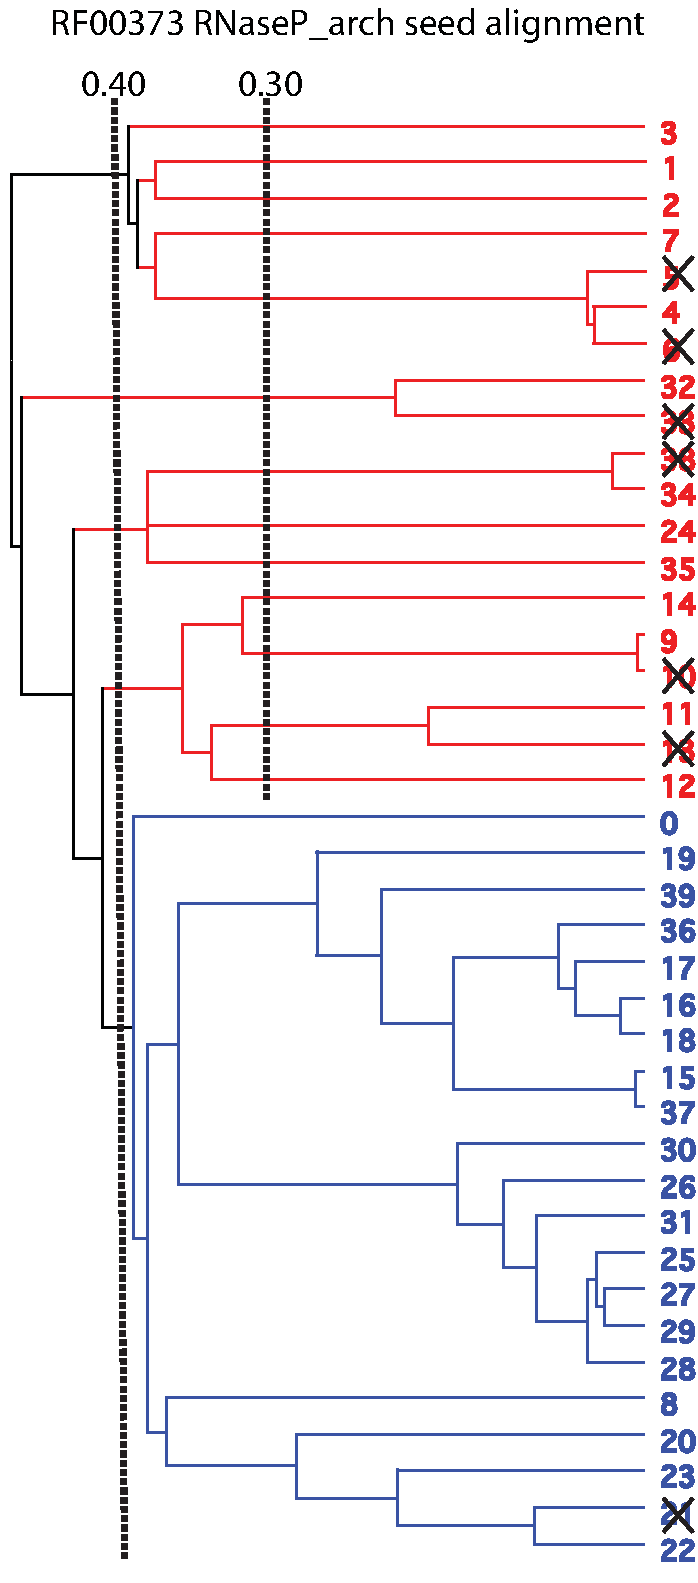
\includegraphics[height=5.5in]{figs/u8-RF00373-tree}

\end{center}
\end{minipage}
\end{slide}
%%%%%%%%%%%%%%%%%%%%%%%%%%%%%%%%%%%%%%%%%%%%%%%%%%%%%%%%%%%%%%%%%%%%%%
\begin{slide}
\begin{center}

\textbf{Infernal outperforms primary-sequence based methods on our
  benchmark (and others\footnote{Freyhult EK, Bollback JP, Gardner
    PP. Genome Res. 2007 17: 117-125.}, not shown)}

\end{center}
\medskip

\center{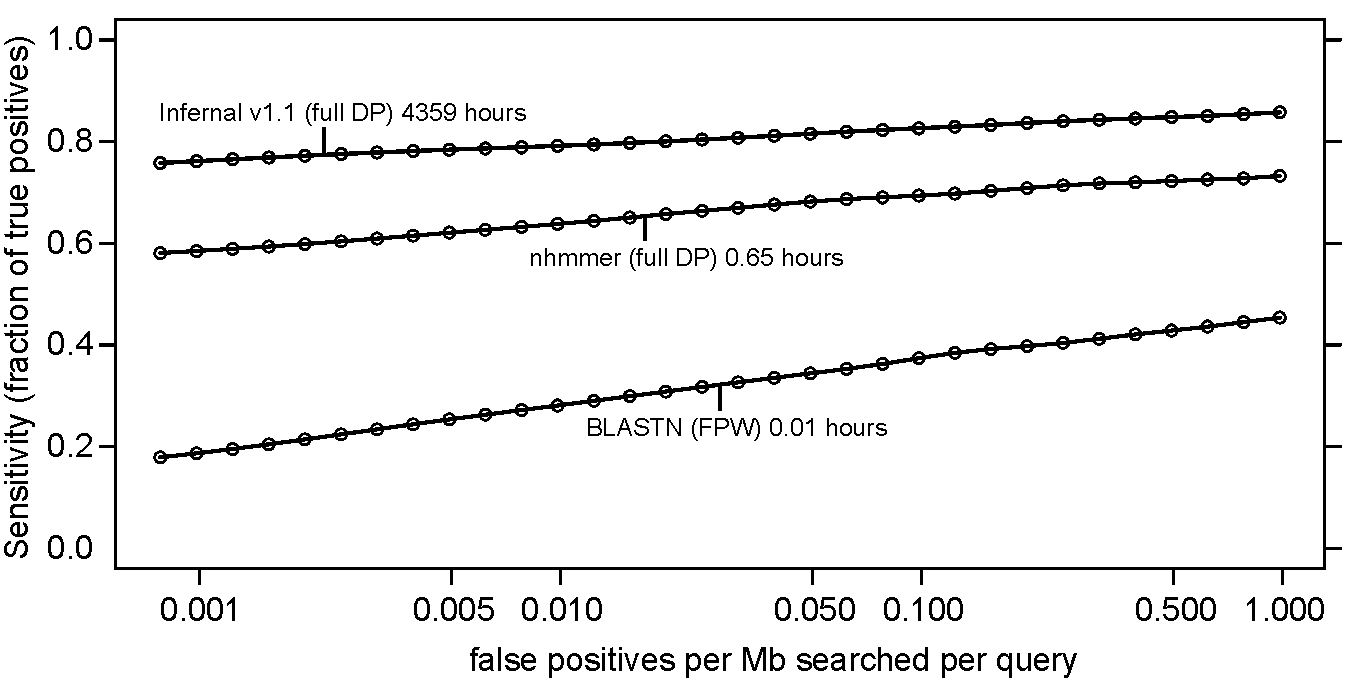
\includegraphics[width=10in]{figs/roc1-jsm}}

\vfill 
\end{slide}
%%%%%%%%%%%%%%%%%%%%%%%%%%%%%%%%%%%%%%%%%%%%%%%%%%%%%%%%%%%%%%%%%%%%%%
\begin{slide}
\begin{center}

\textbf{Over the last several years we've accelerated
  \\ HMMER\footnote{Wheeler TJ, and Eddy SR. Bioinformatics, 29:2487-
    2489, 2013 and Eddy, SR. PLoS Comp. Biol., 7:e1002195, 2011.} and
  Infernal\footnote{Nawrocki EP, Eddy,
    SR. Bioinformatics 2013 29:2487-2489.} by several orders of magnitude}
\end{center}
\medskip

\center{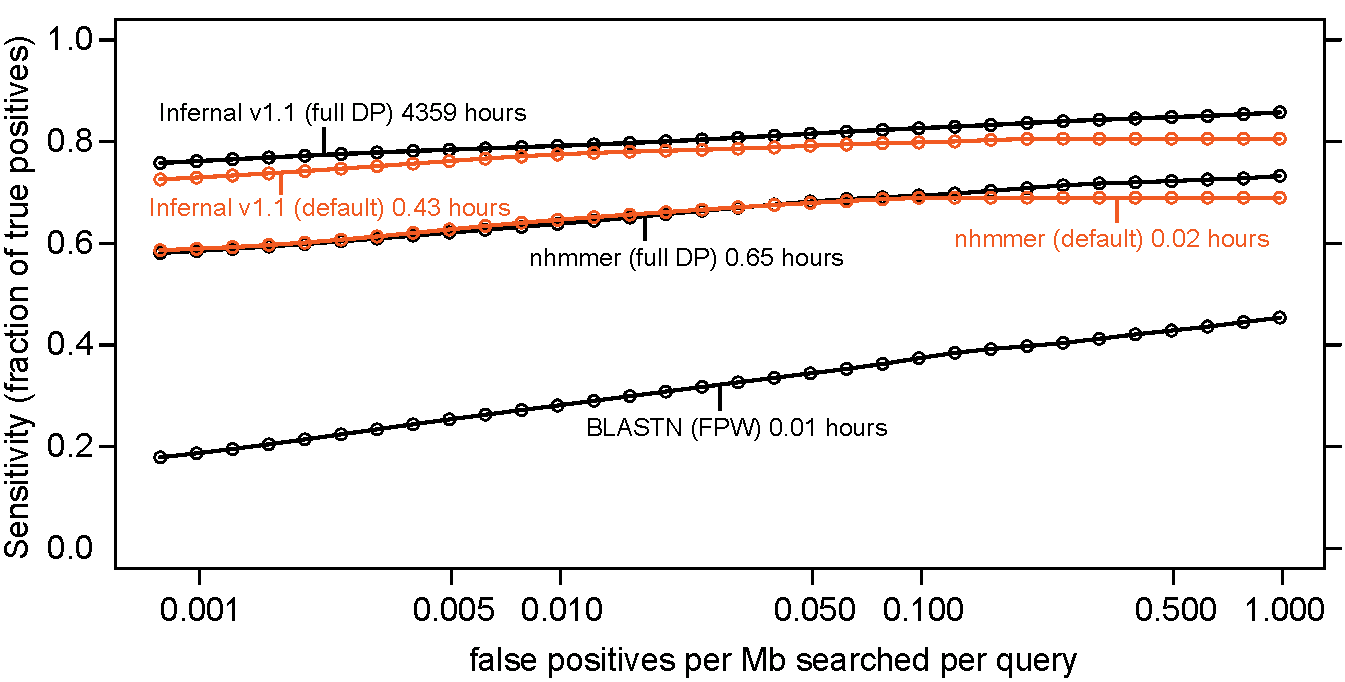
\includegraphics[width=10in]{figs/roc2-jsm}}

\vfill 
\end{slide}
%%%%%%%%%%%%%%%%%%%%%%%%%%%%%%%%%%%%%%%%%%%%%%%%%%%%%%%%%%%%%%%%%%%%%%
\begin{slide}
\begin{center}
\textbf{MSV filter for faster profile HMM searches}
\end{center}

\medskip

\begin{itemize}

\small
\item MSV (Multiple Segment Viterbi) algorithm, which disallows inserts
  and deletes, can be computed using 16-fold vector parallelism with
  low-precision (8-bit) scores\footnote{Eddy SR. PLoS Comp. Biol., 7:e1002195, 2011}.

\end{itemize}

\center{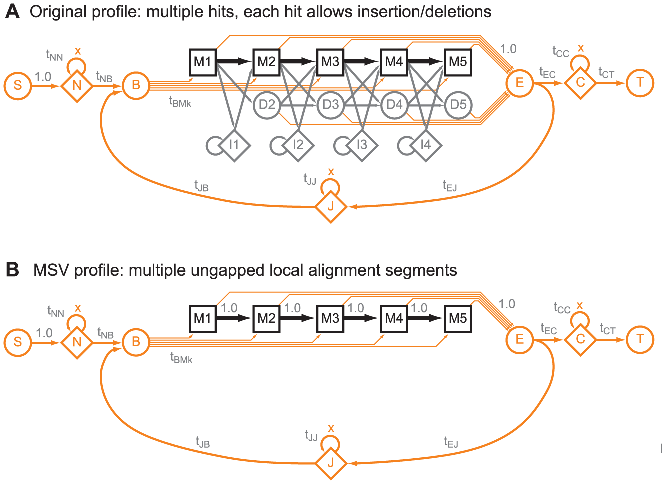
\includegraphics[height=4in]{figs/msv-trunc}}

\vfill 
\end{slide}
%%%%%%%%%%%%%%%%%%%%%%%%%%%%%%%%%%%%%%%%%%%%%%%%%%%%%%%%%%%%%%%%%%%%%%
\begin{slide}
\begin{center}
\textbf{Accelerating Infernal}
\end{center}

\medskip

\begin{itemize}
\item First stage: HMMER's MSV filter with more permissive cutoffs

\item Second stage: align surviving sequence to a profile HMM

\item Third stage: align to CM using constraints from HMM alignment
\end{itemize}

\vfill 
\end{slide}
%%%%%%%%%%%%%%%%%%%%%%%%%%%%%%%%%%%%%%%%%%%%%%%%%%%%%%%%%%%%%%%%%%%%%%%%%%
%%%%%%%%%%%%%%%%%%%%%%%%%%%%%%%%%%%%%%%%%%%%%%%%%%%%%%%%%%%%%%%%%%%%%%%%%%
\begin{slide}
\begin{center}

\textbf{Optimal alignment to an HMM}

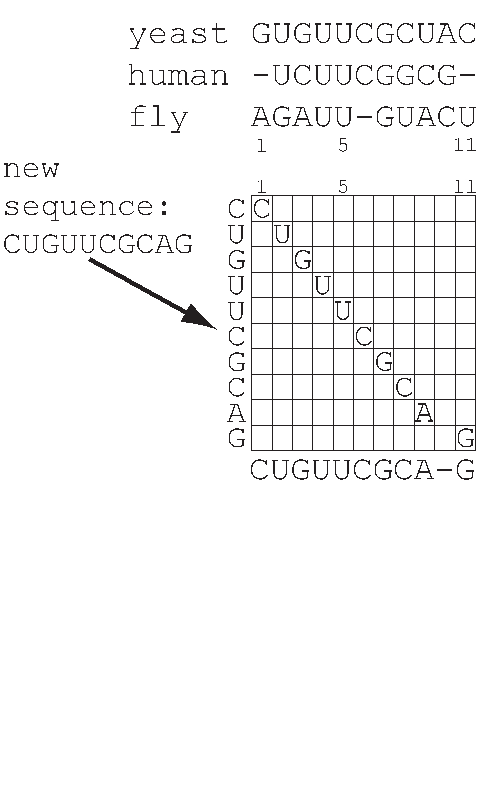
\includegraphics[height=6in]{figs/hmm_alignment2_layer2}
\end{center}

\vfill
\end{slide}
%%%%%%%%%%%%%%%%%%%%%%%%%%%%%%%%%%%%%
%%%%%%%%%%%%%%%%%%%%%%%%%%%%%%%%%%%%%%%%%%%%%%%%%%%%%%%%%%%%%%%%%%%%%%%%%%
\begin{slide}
\begin{center}

\textbf{Posterior decoding of an HMM alignment gives confidence estimates}

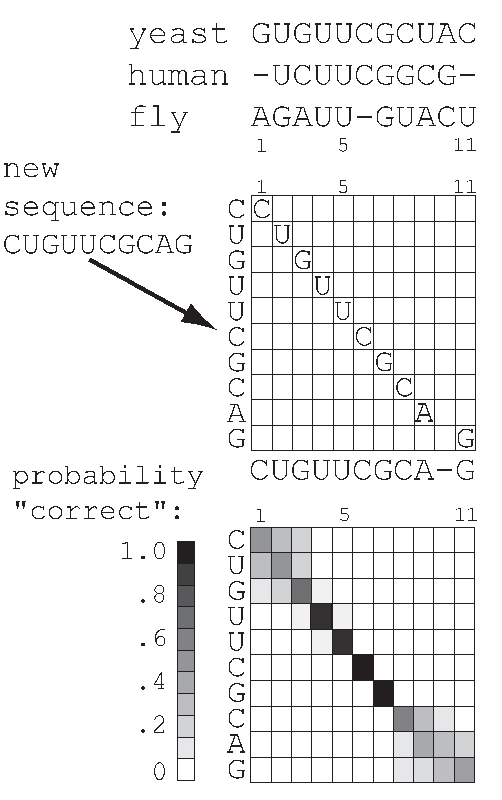
\includegraphics[height=6in]{figs/hmm_alignment2_layer3}
\end{center}

\vfill
\end{slide}
%%%%%%%%%%%%%%%%%%%%%%%%%%%%%%%%%%%%%
\begin{slide}
\begin{center}

\textbf{HMM bands accelerate CM alignment}
\end{center}
\medskip
\small
\begin{itemize}
\item
\textbf{main idea:} eliminate potential alignments the HMM tells us are very improbable
\end{itemize}
\begin{center}
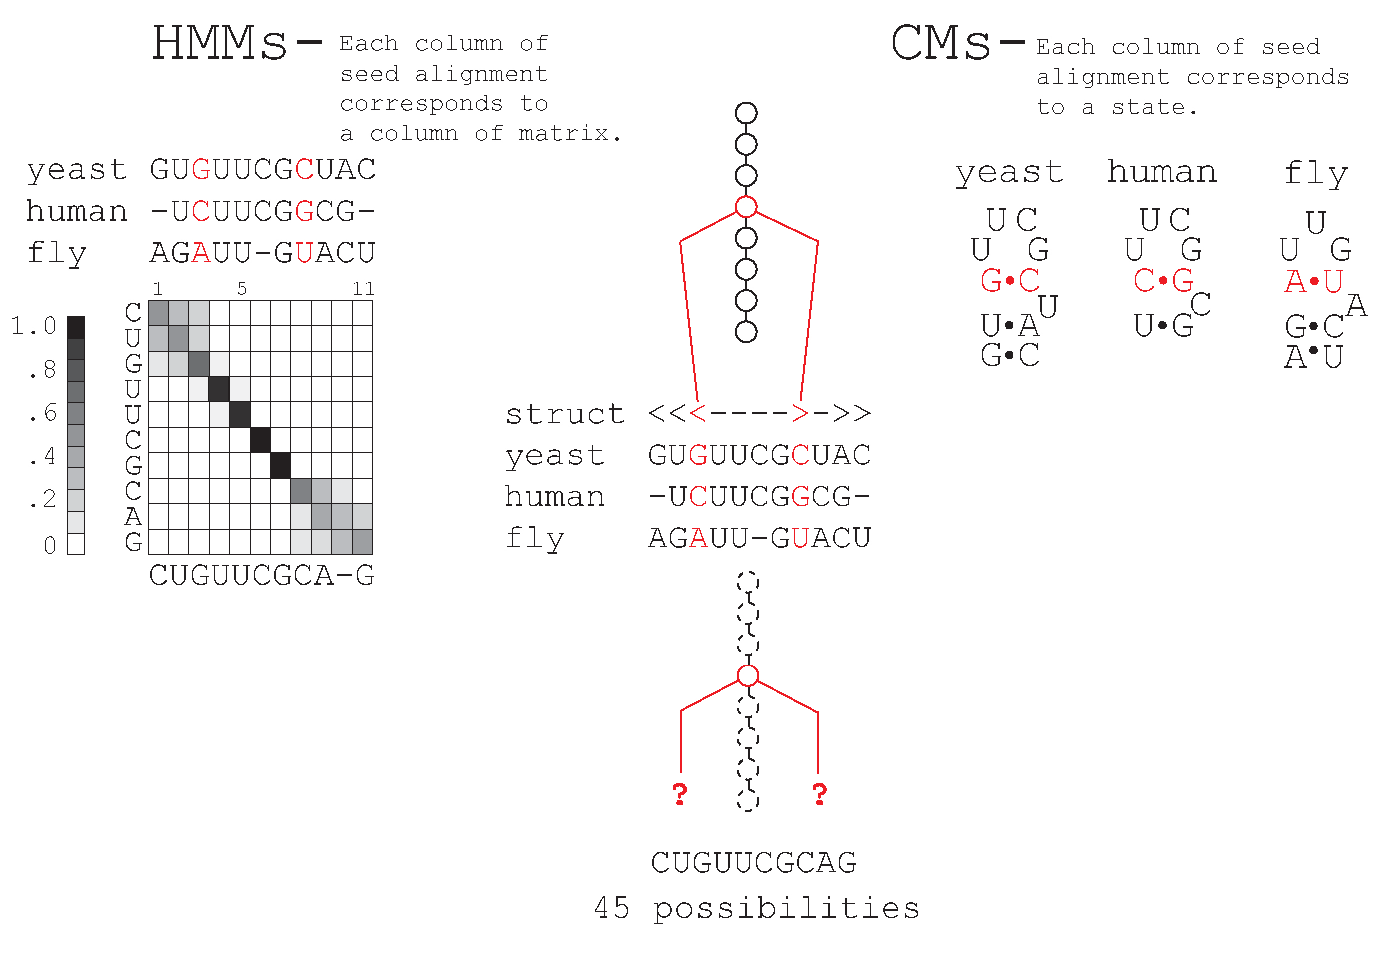
\includegraphics[width=8in]{figs/post_hmm_to_cm_map2_layer14}
\end{center}
\vfill
\end{slide}
%%%%%%%%%%%%%%%%%%%%%%%%%%%%%%%%%%%%%%%%%%%%%%%%%%%%%%%%%%%%%%%%%%%%%%
\begin{slide}
\begin{center}

\textbf{HMM bands accelerate CM alignment}
\end{center}
\medskip
\small
\begin{itemize}
\item
\textbf{main idea:} eliminate potential alignments the HMM tells us are very improbable
\end{itemize}
\begin{center}
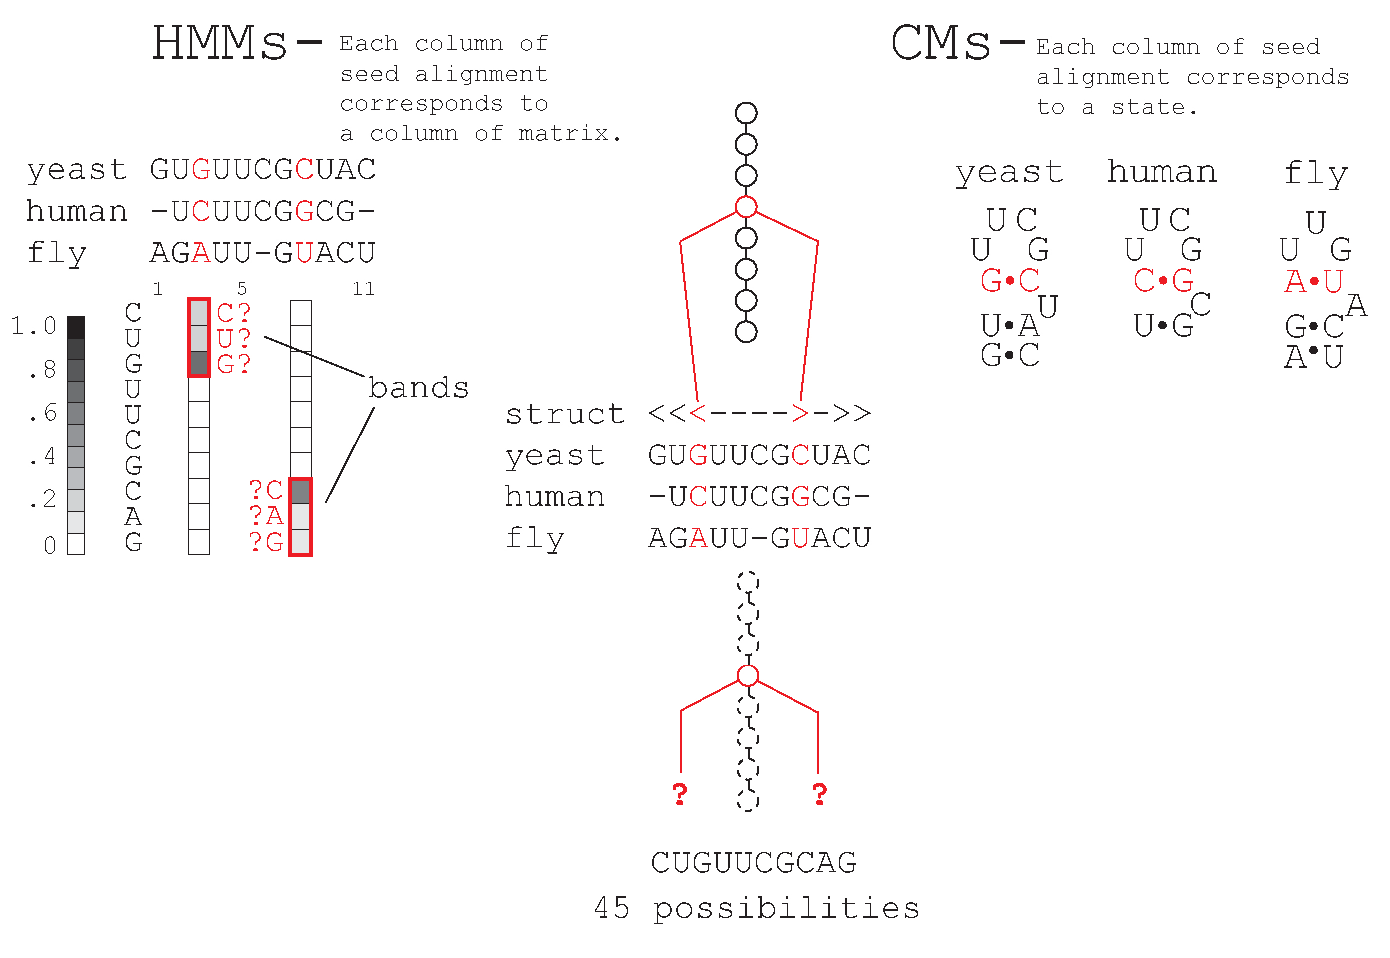
\includegraphics[width=8in]{figs/post_hmm_to_cm_map2_layer15}
\end{center}
\vfill
\end{slide}
%%%%%%%%%%%%%%%%%%%%%%%%%%%%%%%%%%%%%%%%%%%%%%%%%%%%%%%%%%%%%%%%%%%%%%%%%%
%%%%%%%%%%%%%%%%%%%%%%%%%%%%%%%%%%%%%%%%%%%%%%%%%%%%%%%%%%%%%%%%%%%%%%%%%%
\begin{slide}
\begin{center}

\textbf{HMM bands accelerate CM alignment}
\end{center}
\medskip
\small
\begin{itemize}
\item
\textbf{main idea:} eliminate potential alignments the HMM tells us are very improbable
\end{itemize}
\begin{center}
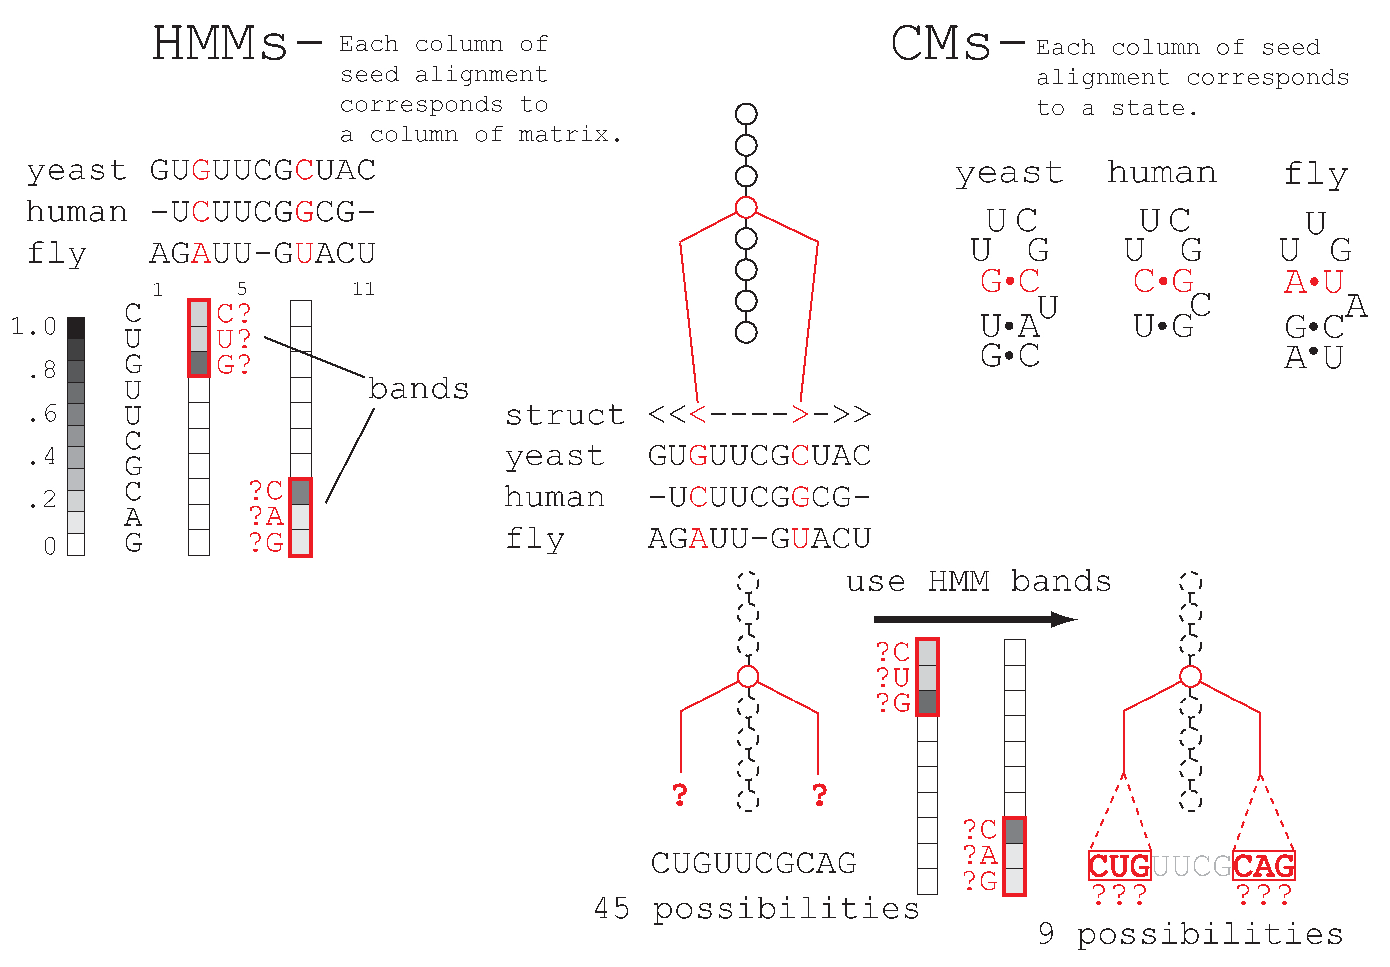
\includegraphics[width=8in]{figs/post_hmm_to_cm_map2_layer16}
\end{center}
\vfill
\end{slide}
%%%%%%%%%%%%%%%%%%%%%%%%%%%%%%%%%%%%%%%%%%%%%%%%%%%%%%%%%%%%%%%%%%%%%%%%%%
%%%%%%%%%%%%%%%%%%%%%%%%%%%%%%%%%%%%%%%%%%%%%%%%%%%%%%%%%%%%%%%%%%%%%%%%%%
\begin{slide}

\large
\begin{center}
\large{\textbf{Acknowledgements}} \\

%\normalsize
%\begin{tabular}{l}
%Sean Eddy           \\
%Travis Wheeler      \\
%Elena Rivas         \\
%Tom Jones           \\
%Diana Kolbe         \\
%Seolkyoung Jung     \\
%Sergi Castellano    \\
%Fred Davis          \\
%Lee Henry           \\
%Michael Farrar      \\
%\end{tabular}

\includegraphics[width=10.5in]{figs/acknowledgements-2014}

\end{center}

\vfill
\end{slide}
%%%%%%%%%%%%%%%%%%%%%%%%%%%%%%%%%%%%%%%%%%%%%%%%%%%%%%%%%%%%%%%
\end{document}



%%%%%%%%%%%%%%%%%%%%%%%%%%%%%%%%%%%%%%%%%%%%%%%%%%%%%%%%%%%%%%%%%%%%%%
\begin{slide}
\begin{center}
\textbf{Vault: a eukaryotic organelle} 
\end{center}
\medskip

\small
\begin{itemize}
\item 
  conserved amongst most eukaryotes
\item 
  function is poorly understood; may play role in fighting pathogens
\item 
  made up of three proteins: major vault protein (MVP) and two minor
  vault proteins
\item 
  barrel shaped organelle has 8-16 vault RNAs (85-150 nt) inside.
\item 
  vault RNA is Pol-III transcribed; contains A- and B-box internal
  promoters, like tRNA.
\end{itemize}

\center{\includegraphics[height=3in]{figs/vault-wiki}}

\vfill
\end{slide}
%%%%%%%%%%%%%%%%%%%%%%%%%%%%%%%%%%%%%%%%%%%%%%%%%%%%%%%%%%%%%%%%%%%%%%%%%%
\begin{slide}
\begin{center}
\textbf{Vault: a eukaryotic organelle} 
\end{center}
\medskip

\small
\begin{itemize}
\item 
  conserved amongst most eukaryotes
\item 
  function is poorly understood; may play role in fighting pathogens
\item 
  made up of three proteins: major vault protein (MVP) and two minor
  vault proteins
\item 
  barrel shaped organelle has 8-16 vault RNAs (85-150 nt) inside.
\item 
  vault RNA is Pol-III transcribed; contains A- and B-box internal
  promoters, like tRNA.
\end{itemize}

\center{\includegraphics[height=3in]{figs/vault-wiki}}

\vfill
\end{slide}
%%%%%%%%%%%%%%%%%%%%%%%%%%%%%%%%%%%%%%%%%%%%%%%%%%%%%%%%%%%%%%%%%%%%%%%%%%
\begin{slide}
\begin{center}
\textbf{Phylogenetic distribution of major vault protein (MVP)}
\end{center}

\center{\includegraphics[width=9in]{figs/euk-broad-markedup}}

\vfill
\end{slide}
%%%%%%%%%%%%%%%%%%%%%%%%%%%%%%%%%%%%%%%%%%%%%%%%%%%%%%%%%%%%%%%%%%%%%%%%%%
\begin{slide}
\begin{center}
\textbf{MVP in animals}
\end{center}

\center{\includegraphics[height=6.5in]{figs/vault-phylogeny-animals-norna}}

\vfill
\end{slide}
\begin{slide}

\center{\includegraphics[height=8.0in]{figs/screen-vault-rfam11.pdf}}

\vfill
\end{slide}
%%%%%%%%%%%%%%%%%%%%%%%%%%%%%%%%%%%%%%%%%%%%%%%%%%%%%%%%%%%%%%%%%%%%%%%%%%
\begin{slide}

\center{\includegraphics[width=9.5in]{figs/vault-11-ic}}

\vfill
\end{slide}
%%%%%%%%%%%%%%%%%%%%%%%%%%%%%%%%%%%%%%%%%%%%%%%%%%%%%%%%%%%%%%%%%%%%%%%%%%
\begin{slide}

\center{\includegraphics[width=9.5in]{figs/vault-11-mi}}

\vfill
\end{slide}
%%%%%%%%%%%%%%%%%%%%%%%%%%%%%%%%%%%%%%%%%%%%%%%%%%%%%%%%%%%%%%%%%%%%%%%%%%
\begin{slide}

\center{\includegraphics[width=9.5in]{figs/screen-tVault-info}}

\vfill
\end{slide}
%%%%%%%%%%%%%%%%%%%%%%%%%%%%%%%%%%%%%%%%%%%%%%%%%%%%%%%%%%%%%%%%%%%%%%%%%%
\begin{slide}
\begin{center}
\textbf{Phylogenetic distribution of Vault proteins and RNAs}
\end{center}
\medskip

\center{\includegraphics[height=7.2in]{figs/vault-phylogeny-animals-rna}}

\vfill
\end{slide}
%%%%%%%%%%%%%%%%%%%%%%%%%%%%%%%%%%%%%%%%%%%%%%%%%%%%%%%%%%%%%%%%%%%%%%%%%%

%%%%%%%%%%%%%%%%%%%%%%%%%%%%%%%%%%%%%%%%%%%%%%%%%%%%%%%%%%%%%%%%%%%%
\begin{slide}
\begin{center}
\textbf{Emission parameters using a mixture Dirichlet
  prior}\footnote{Durbin et al., \emph{Biological Sequence
      Analysis}, Oxford Univ Press, 1998.}
\end{center}
\medskip

\small

\begin{itemize}
\item probability of generating (emitting) residue $a$ from match state $j$: 

\begin{center}
$e_{M_j} (a) = \sum\limits_k P(k|\mathbf{c}_j) \frac{c_{ja} +
    \alpha_a^{k}}{\sum_{a'} (c_{ja'} + \alpha_a^{k})}$
\end{center}

\item where $\mathbf{c}_j$ are weighted counts of emissions 

\item where $p_k$ are the prior probabilities of the mixture components

\item and $P(k|\mathbf{c}_j)$ are the \emph{posterior mixture coefficients}:

\begin{center}
  $P(k|\mathbf{c}_j) = \frac{p_k P(\mathbf{c}_j|k)}{\sum_{k'}p_{k'}P(\mathbf{c}_j|k')}$
\end{center}

\item 
$P(\mathbf{c}_j|k)$ is the probability of the observed counts
($\mathbf{c}_j$) given the mixture component $k$:

\begin{center}

$P(\mathbf{c}_j|k) = \frac{(\sum_a c_{ja})!}{\prod_a c_{ja}!}
  \frac{\prod_a \Gamma(c_{ja} + \alpha_a^{k})}{\sum_a c_{ja}+\alpha_a^{k}}
  \frac{\Gamma(\sum_a \alpha_a^{k})}{\prod_a \Gamma(\alpha_a{^k})}$

\end{center}

\item Mixture components were estimated from large dataset of
alignment columns, by maximum likelihood (by minimizing the
log probability of $P(k|\mathbf{c}_j)$ given current parameters being
estimated via conjugate gradient descent)\footnote{Sjolander et al,
  Comput Appl Biosci 12: 327-345, 1996.}.

\end{itemize}

\vfill
\end{slide}
%%%%%%%%%%%%%%%%%%%%%%%%%%%%%%%%%%%%%%%%%%%%%%%%%%%%%%%%%%%%%%%%%%%%

%%%%%%%%%%%%%%%%%%%%%%%%%%%%%%%%%%%%%%%%%%%%%%%%%%%%%%%%%%%%%%%%%%%%%%%%%%
\begin{slide}
\begin{center}

\textbf{Accelerating CM alignment using HMMs}
\end{center}
\medskip
\begin{minipage}{6in}
\footnotesize
\begin{itemize}
\item
\textbf{main idea:} use fast HMM when it's accurate, appealing to CM when it's not
\item
need some type of measure of confidence in regions of the HMM alignment

\end{itemize}
\small
\hspace{0.3in}
\underline{HMM alignment}%\hspace{1.5in}---- $>$
\begin{itemize}
\item
each column of the grid corresponds to a \\ column
of the seed alignment
\item
each row of the grid corresponds to a \\ position of the new sequence
\end{itemize}
\vspace{3in}
\end{minipage}
\begin{minipage}{4in}
\begin{center}
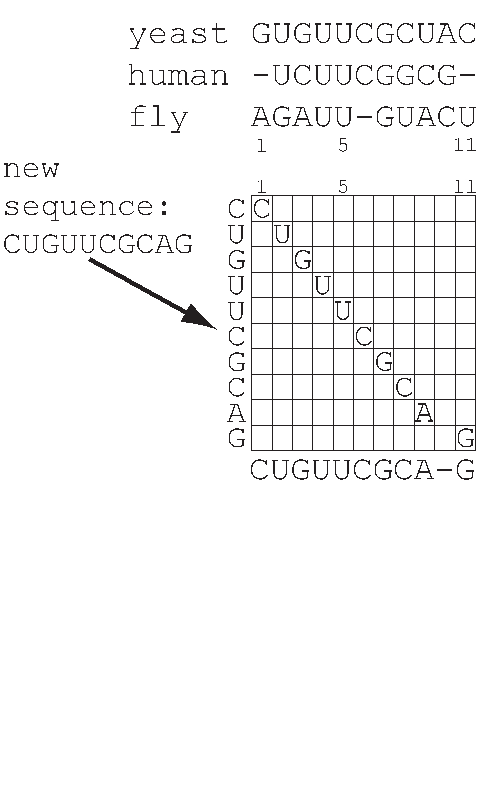
\includegraphics[height=6in]{figs/hmm_alignment2_layer2}
\end{center}
\vspace{1.5in}
\end{minipage}
\end{slide}
%%%%%%%%%%%%%%%%%%%%%%%%%%%%%%%%%%%%%
%%%%%%%%%%%%%%%%%%%%%%%%%%%%%%%%%%%%%%%%%%%%%%%%%%%%%%%%%%%%%%%%%%%%%%%%%%
\begin{slide}
\begin{center}

%\textbf{Accelerating CM alignment using HMMs\footnote{\tiny{this technique
%    was pioneered by Michael Brown in the RNACAD program (Brown MP,
%    Proc. Int. Conf. Intell. Syst. Mol. Biol., 8:57–66, 2000.)}}}
\textbf{Accelerating CM alignment using HMMs}
\end{center}
\medskip
\begin{minipage}{5.5in}
\footnotesize
\begin{itemize}
\item
\textbf{main idea:} use fast HMM when it's accurate, appealing to CM when it's not
\item
need some type of measure of confidence in regions of the HMM alignment

\end{itemize}
\small
\hspace{0.3in}
\underline{HMM alignment}%\hspace{1.5in}---- $>$
\begin{itemize}
\item
each column of the grid corresponds to a \\ column
of the seed alignment
\item
each row of the grid corresponds to a \\ position of the new sequence
\end{itemize}
\vspace{3in}
\end{minipage}
\begin{minipage}{3.5in}
\begin{center}
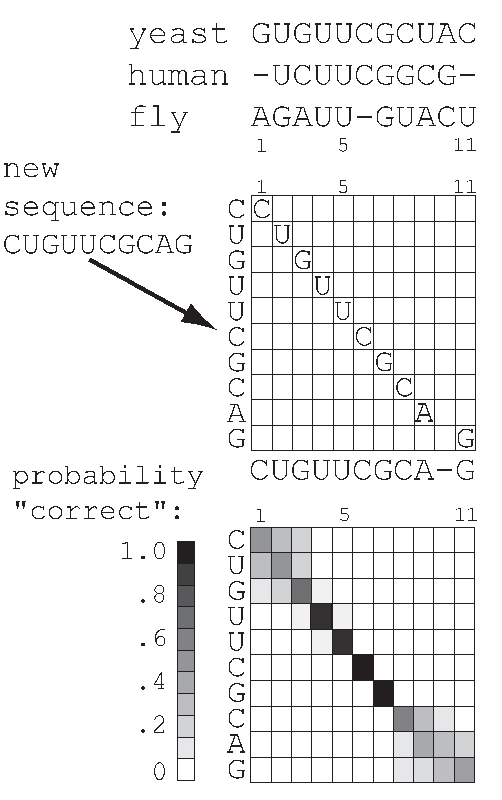
\includegraphics[height=6in]{figs/hmm_alignment2_layer3}
\end{center}
\vspace{1.5in}
\end{minipage}
\end{slide}
%%%%%%%%%%%%%%%%%%%%%%%%%%%%%%%%%%%%%
